%%% The main file. It contains definitions of basic parameters and includes all other parts.

%% Settings for single-side (simplex) printing
% Margins: left 40mm, right 25mm, top and bottom 25mm
% (but beware, LaTeX adds 1in implicitly)
\documentclass[12pt,a4paper]{report}
\setlength\textwidth{145mm}
\setlength\textheight{247mm}
\setlength\oddsidemargin{15mm}
\setlength\evensidemargin{15mm}
\setlength\topmargin{0mm}
\setlength\headsep{0mm}
\setlength\headheight{0mm}
% \openright makes the following text appear on a right-hand page
\let\openright=\clearpage

%% Settings for two-sided (duplex) printing
% \documentclass[12pt,a4paper,twoside,openright]{report}
% \setlength\textwidth{145mm}
% \setlength\textheight{247mm}
% \setlength\oddsidemargin{14.2mm}
% \setlength\evensidemargin{0mm}
% \setlength\topmargin{0mm}
% \setlength\headsep{0mm}
% \setlength\headheight{0mm}
% \let\openright=\cleardoublepage

%% Generate PDF/A-2u
\usepackage[a-2u]{pdfx}

%% Character encoding: usually latin2, cp1250 or utf8:
\usepackage[utf8]{inputenc}

%% Prefer Latin Modern fonts
\usepackage{lmodern}

%% Further useful packages (included in most LaTeX distributions)
\usepackage{amsmath}        % extensions for typesetting of math
\usepackage{amsfonts}       % math fonts
\usepackage{amsthm}         % theorems, definitions, etc.
\usepackage{bbding}         % various symbols (squares, asterisks, scissors, ...)
\usepackage{bm}             % boldface symbols (\bm)
\usepackage{graphicx}       % embedding of pictures
\usepackage{fancyvrb}       % improved verbatim environment
\usepackage{natbib}         % citation style AUTHOR (YEAR), or AUTHOR [NUMBER]
\usepackage[nottoc]{tocbibind} % makes sure that bibliography and the lists
			    % of figures/tables are included in the table
			    % of contents
\usepackage{dcolumn}        % improved alignment of table columns
\usepackage{booktabs}       % improved horizontal lines in tables
\usepackage{paralist}       % improved enumerate and itemize
\usepackage{xcolor}         % typesetting in color

\usepackage{times}
\usepackage{latexsym}
\usepackage{tipa}
\usepackage[normalem]{ulem} % sout
\usepackage[noabbrev,capitalize]{cleveref}
\usepackage{tikz}
\usetikzlibrary{positioning,shapes,arrows,calc,decorations.pathmorphing}
\usepackage{textcomp}
\usepackage{makecell}
\usepackage{enumitem}
\usepackage{pgfplots}
\usepackage{tikzscale}
\usepackage{microtype}
\usepackage{rotating}
\usepackage{pdflscape}
\usepackage{multirow}
\usepackage{tipa}


%%% Basic information on the thesis

% Thesis title in English (exactly as in the formal assignment)
\def\ThesisTitle{Spoken Language Translation via Phoneme Representation of the Source Language}

% Author of the thesis
\def\ThesisAuthor{Peter Polák}

% Year when the thesis is submitted
\def\YearSubmitted{2020}

% Name of the department or institute, where the work was officially assigned
% (according to the Organizational Structure of MFF UK in English,
% or a full name of a department outside MFF)
\def\Department{Institute of Formal and Applied Linguistics}

% Is it a department (katedra), or an institute (ústav)?
\def\DeptType{Institute}

% Thesis supervisor: name, surname and titles
\def\Supervisor{doc. RNDr. Ondřej Bojar, Ph.D.}

% Supervisor's department (again according to Organizational structure of MFF)
\def\SupervisorsDepartment{Institute of Formal and Applied Linguistics}

% Study programme and specialization
\def\StudyProgramme{Computer Science}
\def\StudyBranch{Artificial Intelligence}

% An optional dedication: you can thank whomever you wish (your supervisor,
% consultant, a person who lent the software, etc.)
\def\Dedication{%
Dedication.
}

% Abstract (recommended length around 80-200 words; this is not a copy of your thesis assignment!)
\def\Abstract{%
Abstract.
}

% 3 to 5 keywords (recommended), each enclosed in curly braces
\def\Keywords{%
{key} {words}
}

%% The hyperref package for clickable links in PDF and also for storing
%% metadata to PDF (including the table of contents).
%% Most settings are pre-set by the pdfx package.
\hypersetup{unicode}
\hypersetup{breaklinks=true}

% Definitions of macros (see description inside)
%%% This file contains definitions of various useful macros and environments %%%
%%% Please add more macros here instead of cluttering other files with them. %%%

%%% Minor tweaks of style

% These macros employ a little dirty trick to convince LaTeX to typeset
% chapter headings sanely, without lots of empty space above them.
% Feel free to ignore.
\makeatletter
\def\@makechapterhead#1{
  {\parindent \z@ \raggedright \normalfont
   \Huge\bfseries \thechapter. #1
   \par\nobreak
   \vskip 20\p@
}}
\def\@makeschapterhead#1{
  {\parindent \z@ \raggedright \normalfont
   \Huge\bfseries #1
   \par\nobreak
   \vskip 20\p@
}}
\makeatother

% This macro defines a chapter, which is not numbered, but is included
% in the table of contents.
\def\chapwithtoc#1{
\chapter*{#1}
\addcontentsline{toc}{chapter}{#1}
}

% Draw black "slugs" whenever a line overflows, so that we can spot it easily.
\overfullrule=1mm

%%% Macros for definitions, theorems, claims, examples, ... (requires amsthm package)

\theoremstyle{plain}
\newtheorem{thm}{Theorem}
\newtheorem{lemma}[thm]{Lemma}
\newtheorem{claim}[thm]{Claim}

\theoremstyle{plain}
\newtheorem{defn}{Definition}

\theoremstyle{remark}
\newtheorem*{cor}{Corollary}
\newtheorem*{rem}{Remark}
\newtheorem*{example}{Example}

%%% An environment for proofs

\newenvironment{myproof}{
  \par\medskip\noindent
  \textit{Proof}.
}{
\newline
\rightline{$\qedsymbol$}
}

%%% An environment for typesetting of program code and input/output
%%% of programs. (Requires the fancyvrb package -- fancy verbatim.)

\DefineVerbatimEnvironment{code}{Verbatim}{fontsize=\small, frame=single}

%%% The field of all real and natural numbers
\newcommand{\R}{\mathbb{R}}
\newcommand{\N}{\mathbb{N}}

%%% Useful operators for statistics and probability
\DeclareMathOperator{\pr}{\textsf{P}}
\DeclareMathOperator{\E}{\textsf{E}\,}
\DeclareMathOperator{\var}{\textrm{var}}
\DeclareMathOperator{\sd}{\textrm{sd}}

%%% Transposition of a vector/matrix
\newcommand{\T}[1]{#1^\top}

%%% Various math goodies
\newcommand{\goto}{\rightarrow}
\newcommand{\gotop}{\stackrel{P}{\longrightarrow}}
\newcommand{\maon}[1]{o(n^{#1})}
\newcommand{\abs}[1]{\left|{#1}\right|}
\newcommand{\dint}{\int_0^\tau\!\!\int_0^\tau}
\newcommand{\isqr}[1]{\frac{1}{\sqrt{#1}}}

%%% Various table goodies
\newcommand{\pulrad}[1]{\raisebox{1.5ex}[0pt]{#1}}
\newcommand{\mc}[1]{\multicolumn{1}{c}{#1}}


\def\XXX#1{{\textcolor{red}{XXX #1}}}


% Definition of blocks:
\tikzset{%
	block/.style    = {draw,  rectangle, minimum height = 2.7em,
		minimum width = 3em}
}

\renewcommand{\UrlFont}{\ttfamily\small}

% This is not strictly necessary, and may be commented out,
% but it will improve the layout of the manuscript,
% and will typically save some space.

%\aclfinalcopy % Uncomment this line for the final submission
%\def\aclpaperid{***} %  Enter the acl Paper ID here

%\setlength\titlebox{5cm}
% You can expand the titlebox if you need extra space
% to show all the authors. Please do not make the titlebox
% smaller than 5cm (the original size); we will check this
% in the camera-ready version and ask you to change it back.

\newcommand\BibTeX{B\textsc{ib}\TeX}


\def\XXX#1{{\textcolor{red}{XXX #1}}}
\def\repl#1#2{{\textcolor{red}{\sout{#1}}\textcolor{blue}{#2}}}
\def\parcite#1{\citep{#1}} % (Smith, 2012)
\def\perscite#1{\citet{#1}} % Smith (2012)
\def\inparcite#1{\citealp{#1}} % should be Smith, 2012

\def\footurl#1{\footnote{\url{#1}}}

\newcommand\litem[1]{\item{\bfseries #1}}
\def\tabspace#1{\vline height#1 width0pt\relax}

% Title page and various mandatory informational pages
\begin{document}
%%% Title page of the thesis and other mandatory pages

%%% Title page of the thesis

\pagestyle{empty}
\hypersetup{pageanchor=false}
\begin{center}

\centerline{\mbox{\includegraphics[width=166mm]{img/logo-en.pdf}}}

\vspace{-8mm}
\vfill

{\bf\Large MASTER THESIS}

\vfill

{\LARGE\ThesisAuthor}

\vspace{15mm}

{\LARGE\bfseries\ThesisTitle}

\vfill

\Department

\vfill

{
\centerline{\vbox{\halign{\hbox to 0.45\hsize{\hfil #}&\hskip 0.5em\parbox[t]{0.45\hsize}{\raggedright #}\cr
Supervisor of the master thesis:&\Supervisor \cr
\noalign{\vspace{2mm}}
Study programme:&\StudyProgramme \cr
\noalign{\vspace{2mm}}
Study branch:&\StudyBranch \cr
}}}}

\vfill

% Zde doplňte rok
Prague \YearSubmitted

\end{center}

\newpage

%%% Here should be a bound sheet included -- a signed copy of the "master
%%% thesis assignment". This assignment is NOT a part of the electronic
%%% version of the thesis. DO NOT SCAN.
This is not a~part of the electronic version of the thesis, do not scan!

%%% A page with a solemn declaration to the master thesis

\openright
\hypersetup{pageanchor=true}
\pagestyle{plain}
\pagenumbering{roman}
\vglue 0pt plus 1fill

\noindent
I declare that I carried out this master thesis independently, and only with the cited
sources, literature and other professional sources. It has not been used to obtain another
or the same degree.

\medskip\noindent
I understand that my work relates to the rights and obligations under the Act No.~121/2000 Sb.,
the Copyright Act, as amended, in particular the fact that the Charles
University has the right to conclude a license agreement on the use of this
work as a school work pursuant to Section 60 subsection 1 of the Copyright~Act.

\vspace{10mm}

\hbox{\hbox to 0.5\hsize{%
In \hbox to 6em{\dotfill} date \hbox to 6em{\dotfill}
\hss}\hbox to 0.5\hsize{\dotfill\quad}}
\smallskip
\hbox{\hbox to 0.5\hsize{}\hbox to 0.5\hsize{\hfil Author's signature\hfil}}

\vspace{20mm}
\newpage

%%% Dedication

\openright

\noindent
\Dedication

\newpage

%%% Mandatory information page of the thesis

\openright

\vbox to 0.5\vsize{
\setlength\parindent{0mm}
\setlength\parskip{5mm}

Title:
\ThesisTitle

Author:
\ThesisAuthor

\DeptType:
\Department

Supervisor:
\Supervisor, \SupervisorsDepartment

Abstract:
\Abstract

Keywords:
\Keywords

\vss}

\newpage

\openright
\pagestyle{plain}
\pagenumbering{arabic}
\setcounter{page}{1}

%%% A page with automatically generated table of contents of the master thesis

\tableofcontents

%%% Each chapter is kept in a separate file
\chapter*{Introduction}
\addcontentsline{toc}{chapter}{Introduction}

\section*{Work organization}
We settled on a less traditional strategy for the organization of this work: we serve every chapter as a standalone small paper. Notably, each chapter includes a section about related work devoted to the chapter's subject. We review mutual related work in \cref{chap:theory} (such as neural network architectures or corpora).

Chapters progressively deal with problematic starting with Automatic Speech Recognition in \cref{chapter:asr}, further enhancing ASR in \cref{chap:enhanced_asr}, continuing with Spoken Language Translation in \cref{chap:slt}. Adaptation to speaker is described in \cref{chap:adaptation}. We also deal with ``bringing our work to life'' in \cref{chap:onlinezation}. Finally, we conclude the work in \cref{chap:conclusion}.

\chapter{Tasks, Architectures, and Datasets}
\label{chap:theory}

In this chapter, we give a brief overview of the theoretical foundations for this thesis. First, we define the main tasks that are part of the solution. Further, we describe the utilized neural network architectures. Lastly, we describe used data sets and introduce evaluation metrics.

\section{Automatic Speech Recognition}

Automatic Speech Recognition (ASR) is one of the most popular tasks in NLP. With ever-growing technology that becomes more and more integrated with our day-to-day life, it is clear that ASR will play an essential role in this process.

In this section, we first briefly review the history and then describe the most popular contemporary approaches to ASR.

\subsection{Brief History}

The first attempts for ASR systems stem from the 1950s. Early ASR systems worked with syllables, vowels, and phonemes \parcite{juang2005automatic}. For example, a spoken digit recognizer from Bell laboratories. Their system estimated formant frequencies (as a vowel is pronounced, vocal tract sounds with natural modes of resonance called a formant) of vowel regions of an isolated digit. 

A big leap in ASR systems was the introduction and popularization of Hidden Markov models (HMMs) in the 1980s. HMMs caused architecture to shift from pattern recognition to statistical modeling. The success of HMM-based ASR systems continues even today in the form of hybrid models consisting of HMMs and either Gaussian Mixture Models (GMMs) or Artificial Neural Networks (ANNs).

In the last few years, deep neural networks (DNNs) gained much popularity. In many tasks, ranging from image processing to natural language processing, DNNs outperformed other known methods. Besides their performance, they tend to require less expertise and engineering skills for a particular task than other methods. This makes them available for researchers in many areas. DNNs are becoming a standard in ASR currently, but the first attempts were already made briefly after the introduction of the backpropagation algorithm \parcite{rumelhart1986learning}. They were used for recognition of phonemes \parcite{waibel1989phoneme} or short sequences of words \parcite{lubensky1988learning}. Further important milestones for ASR were recurrent neural networks and attention (applied, for example, in \perscite{chorowski2014end}).

\subsection{Models}
In this section, we introduce contemporary models utilized for ASR. There are two such approaches: (1) HMM-based models, (2) End-to-End neural models.

\subsubsection{HMM-based Models}
HMMs (Hidden Markov Models) are probably the most used technique in ASR \parcite{padmanabhan2015machine,yu2016automatic}. Hidden Markov Models capture the speech sequence as sequence of oservations. In the ASR context, HMMs utilize either GMMs or ANNs in order to model frame-based speech features (features with no temporal information). Practitioners often refer to the HMM-based models combined with neural networks as hybrid models.

A typical pipeline of an HMM-based model works as follows: the input is first pre-processed and converted to features, typically the MFCCs (see \cref{mfcc}). These features are further passed to the estimator. Common unit in a HMM-based pipeline is \emph{phone}. The decoder employs an \emph{acoustic model}, a \emph{dictionary} and a \emph{language model} to decode the speech. The acoustic model estimates the probability of the acoustic sequence given word sequence. ANNs or GMMs represent the acoustic model. Dictionary maps phone sequences to words. Finally, the language model estimates the apriori probability of word sequence, independent of the observed sound. Commonly, $n$-gram language models are used. 

\subsubsection{End-to-End Models}
The alternative to the HMM-based models are End-to-End (E2E) ASR pipelines. The common trait for these models is their ability to produce the final, human-readable text given acoustic features using one end-to-end deep neural network. Recent advancements (such as \perscite{amodei2016deep,Li2019}) clearly show the future direction towards this kind of ASR. The advantage of E2E models is that they require less engineering than HMM models. An open problem remains the higher requirement of training data.

The input of the model are commonly MFCC features extracted from speech data. E2E models use two approaches: Connectionist temporal classification (CTC) \parcite{graves2006connectionist} loss (e.g., \perscite{hannun2014deep,zhang2017towards}) or attention mechanism (e.g., \perscite{bahdanau2016end}). The inference algorithms include a conventional beam search with the language model (LM) (again, an $n$-gram LM is used) that re-scores the beams during the decoding. The use of LM in the beam search further enhances the transcription quality.






\pagebreak
\section{Spoken Language Translation}
Spoken Language Translation is another NLP task dealing with speech processing. In literature, the SLT task describes translation into a target language text. Commonly, SLT can also be a speech-to-speech translation. Traditional layout of speech translation, before the emergence of end-to-end systems, consisted of a speech recognition unit followed by machine translation. With the upraise of deep learning, E2E frameworks that do not need intermediate transcription step are gaining popularity \parcite{berard2016listen,berard2018end,jia2019leveraging}.

Direct comparison of both approaches to date seems inconclusive \parcite{sperber2019attention}. Also, the E2E and cascaded SLT differ: E2E SLT must be trained on corpora consisting od source speech and target text (``E2E corpora''), while the cascading can be trained on independent corpora of speech and transcripts for ASR and independently parallel corpora for MT. This makes the latter suitable in cases where there is no corpus for a given language pair available (which is mostly the case). On the other hand, cascading speech recognition and machine translation for SLT often introduces errors in source language transcription that are further propagated to final translation.






\pagebreak
\section{Neural Network Architectures and Models}
In this section, we introduce neural network architectures and models we engage in our work. The first two models, Jasper and QuartzNet, are used as acoustic models. Finally, we present Transformer, which serves as a translation and transcript correction model.

\subsection{Jasper}

Jasper \parcite{Li2019} is a family of end-to-end, deep convolutional neural network ASR architectures.

\subsubsection{Architecture Overview}
The input of the model are MFCCs (Mel Frequency Cepstrum Coefficients, see \cref{mfcc}) obtained from 20 ms frames with 10 ms stride. We use 64 features. The model outputs the probability over a given vocabulary for every processed frame. In our ASR pipeline, the vocabulary is IPA phonemes.

The input is passed through one pre-processing layer, followed by the central part of the network. Finally, tree post-processing layers are applied. The central part of the model consists of so-called ``blocks''.

The Jasper model consists of $B$ blocks and $R$ sub-blocks. Jasper authors introduce a naming convention where such model is described as ``Jasper $B$x$R$''. In our experiments, we use Jasper 10x5.

Each sub-block applies operations as follows: 1D convolution, ReLU activation, and dropout. All sub-blocks of a block have the same number of output channels. 

Further, Jasper's authors observed that models deeper than Jasper 5x3 require residual connections to converge. Residual connections inspired by DenseNet \parcite{huang2017densely} and DenseRNet \parcite{tang2018acoustic} are employed.

The input of a block is connected to its last sub-block via residual connections. Because the number of channels differs, 1x1 convolution is applied to account for this. After this projection, batch normalization is applied. The output is then added to the output of the batch normalization layer in the last sub-block. Afterward, the activation function and dropout are used, producing the output of the current block.

The schema of Jasper with residual connections is provided in \cref{fig:jasper_dr}. The biggest used configuration for English graphemes has 333 million parameters.

\begin{figure}[]
	\centering
	\includegraphics[width=0.9\linewidth]{img/JasperVerticalDR4.png}
	\caption{Jasper Dense Residual, taken from \perscite{li2019jasper}.}
	\label{fig:jasper_dr}
\end{figure}

\subsection{QuartzNet}
\label{intro:quartznet}

QuartzNet \parcite{kriman2019quartznet} is another end-to-end ASR architecture used in our work. QuartzNet is a convolutional neural network based on Jasper \parcite{Li2019} architecture having a fraction of parameters (18.9 million versus 333 million) while still achieving near state-of-the-art accuracy.

Same as for the Jasper model, the network's input is 64 MFCC features computed from windows of length 20 ms and overlap 10 ms. The network outputs probability over the given alphabet for each time frame. For training is used CTC loss and for decoding beam search.

The main difference between QuartzNet and Jasper is the application of 1D time-channel separable convolutions.  Such convolutions can be separated into 1D depthwise convolutional layers with kernel $K$ and a pointwise convolution operating across all channels on each time frame independently. A standard 1D convolutional layer with kernel size $K$ and $c_{in}$ input and $c_{out}$ output channels has $K \times c_{in} \times c_{out}$ weights. On the other hand, the 1D depthwise convolution with kernel $K$ has $K \times c_{in}$ weights followed by the pointwise convolution with $c_{in} \times c_{out}$ weights --- together yielding $K \times c_{in} + c_{in} \times c_{out}$ weights. Because of this, the model has fewer parameters and can even have $3 \times$ larger kernel than the bigger Jasper model. The architecture schema is in \cref{fig:quartz_arch}.

The authors describe a further reduction of weights by using grouped pointwise convolution instead of the pointwise convolution layer (see  \cref{fig:quartz_arch_groups}). When using four groups, the number of parameters is halved (for QuartzNet-15x5 from 18.9M to 8.7M) with slightly worse performance (WER 3.98 increases to 4.29 for LibriSpeech dev clean and 11.58 increases to 13.48).

As the first described weights reduction is sufficient for our purposes, we work with QuertzNet without the grouped pointwise convolution.

\begin{figure}[]
	\centering
	\includegraphics[width=0.9\linewidth]{img/QuartzNet_v2.png}
	\caption{QuartzNet BxR architecture. Taken from \perscite{kriman2019quartznet}.}
	\label{fig:quartz_arch}
\end{figure}

\begin{figure}[]
	\centering
	\includegraphics[width=0.8\linewidth]{img/QuartzNet_Grouped_v2.png}
	\caption{(a) Time-channel separable 1D convolutional module (b) Time-channel separable 1D convolutional module with groups and shuffle. Taken from \perscite{kriman2019quartznet}.}
	\label{fig:quartz_arch_groups}
\end{figure}



\subsection{Transformer}
Transformer \parcite{vaswani2017attention} has become a very well established architecture in Neural Machine Translation \parcite{bojar2018proceedings,barrault2019findings}. The main idea behind the architecture is to get rid of recurrence and convolutions and rather base the model solely on attention. As the attention mechanism is implemented as matrix multiplications, contemporary GPUs can better parallelize the computations leading to faster training.

A Transformer model is composed of a encoder and a decoder (see \cref{fig:transformer}). Both encoder and decoder are stacked identical layers. The encoder layer has two sub-layers: a multi-head self-attention layer and a fully connected feed-forward network. Decoder layer has an extra multi-head attention sub-layer, which performs attention over the output of the encoder. This additional layer is between the self-attention and feed-forward layers. Self-attention in the decoder is modified so that the auto-regressive property holds, i.e., the encoder cannot look to the right side (``future'').

The advantage of self-attention is that it can access an arbitrary position in a constant number of sequentially executed operations while recurrent networks need $O(n)$ sequentially executed operations. If the sequence length $n$ is less than the representation dimension $d$ of the model, which is often the case (as the state-of-the-art machine translation models use sub-word units), the total computational complexity is lower than of the recurrent models. Another advantage presented by the authors is that self-attention leads to better interpretability of the models. They claim the individual attention heads seem to learn some specific functions that may be related to the syntactic and semantic structure of a sentence.

We employ this model in our enhanced ASR pipeline as a correction and language model and as a translation model in our SLT pipeline. 


\begin{figure}[]
	\centering
	\includegraphics[width=0.8\linewidth]{img/ModalNet-21.png}
	\caption{Transformer model architecture with detailed encoder (left) and decoder (right). Taken from \perscite{vaswani2017attention}}
	\label{fig:transformer}
\end{figure}





\pagebreak
\section{Data Representation}
This section introduces the input and output data representations. The way how we encode and feed the neural network can significantly influence performance. In this work, we transcribe recordings, i.e., we work with voice and text data. First, we introduce MFCC --- the voice presentation, and then we discuss text encoding.

\subsection{MFCC}
\label{mfcc}
Mel frequency cepstral coefficients (MFCC) is the most commonly used representation of speech for ASR and SLT. 
This method exploits the way how the human auditory system perceives voice. The filter in the MFCC pipeline is linearly spaced for frequencies up to 1000 Hz and logarithmically above. 

MFCC pipeline as described in \perscite{muda2010voice} and \perscite{kamath2019deep}:

\begin{enumerate}
	\litem{Pre-emphasis} Application of filter that emphasizes higher frequencies:
	
	\begin{equation}
	Y[n] = X[n] - \alpha X[n-1]
	\end{equation}.
	
	The $\alpha$ coefficient is typically between 0.95 and 0.99.  This filter amplifies the higher frequencies of the signal.
	
	\litem{Framing} Raw audio is segmented into small windows. The signal within each of the small windows can be then treated as stationary. Typically, the length of the window is about 20 ms, and windows have an overlap of 10 ms.
	
	\litem{Windowing} To avoid potential abrupt changes caused by framing, windowing is applied. Windowing is a multiplication of samples in a window with a scaling function. The most commonly used windowing in ASR is that of Hann and Hamming:
	\begin{equation}
	w(n) = \sin^2{\left( \frac{\pi n}{N - 1} \right)}
	\end{equation}
	\begin{equation}
	w(n) = 0.54 - 0.46 \cos{\left(\frac{2\pi n}{N - 1}\right)}
	\end{equation}
	where $N$ is window length and $0 \leq n \leq N - 1$.
	
	\litem{Fast Fourier Transform} FFT converts the one-dimensional signal from the time to the frequency domain.
	
	\litem{Mel Filter Bank}
	The Mel Filter Bank is a set of filters that mimic the human auditory system. Usually, 40 filters are used. Each filter is of a triangular shape. Each filter produces the weighted sum of the spectral frequencies corresponding to each filter. These values map the input frequencies to the mel scale (a perceptual scale of pitches judged by listeners to be equal in distance from one another proposed by \perscite{stevens1937scale}).
	
	\litem{Discrete Cosine Transform} This process converts the log Mel spectrum into the time domain. The result is called the Mel Frequency Cepstrum Coefficient (the MFCC), and the set of coefficients is called acoustic vectors.
\end{enumerate}

An example of a mel-spectrogram is in \cref{fig:mel}.

\begin{figure}[h!b]
	\centering
	\begin{subfigure}[t]{.49\textwidth}
		\centering
		\includegraphics[width=.8\linewidth]{img/mel_amplitude}
		\caption{Amplitude}
		\label{fig:sfig1}
	\end{subfigure}%     
	\hfill
	\begin{subfigure}[t]{.49\textwidth}
		\centering
		\includegraphics[width=.8\linewidth]{img/mel_jasper}
		\caption{Mel filters: 64; window: 20~ms; overlap: 10~ms; window: hann. (Jasper defaults).}
		\label{fig:sfig2}
	\end{subfigure}
	\begin{subfigure}[b]{.49\textwidth}
		\centering
		\includegraphics[width=.8\linewidth]{img/mel2}
		\caption{Mel filters: 64; window: 20~ms; overlap: 10~ms; window: rectangular.}
		\label{fig:sfig3}
	\end{subfigure}
     \hfill
	\begin{subfigure}[b]{.49\textwidth}
	\centering
	\includegraphics[width=.8\linewidth]{img/mel}
	\caption{Mel filters: 256; window: 50~ms; overlap: 0~ms; window: hann.}
	\label{fig:sfig4}
\end{subfigure}
	\caption{Amplitude and mel spectograms of ``Hello World!''.}
	\label{fig:mel}
\end{figure}

\clearpage

\subsection{Text Representation in NMT}
\label{intro:text_repre}

There are many approaches to text representation in NMT. The first decision that has to be made is the size of the basic text unit. Text can be treated as a sequence of atomic:

\begin{itemize}
	\item characters,
	\item words,
	\item sub-word units.
\end{itemize}

The first one is a very simple and straightforward approach. Character representation permits one to encode any word (of a given alphabet). Its downside is that it produces longer sequences compared with other methods. Less output classes lead to the reduction of computational complexity. However, the model needs to attend more positions, which substantially increases time complexity during decoding.

Word level representation, on the other hand, produces shorted sequences which may be better in some applications. Generally, though, neural machine translation is an open-vocabulary problem. From this point of wiev, word-level representation is undesirable, because it cannot handle unknown words. Several techniques have been proposed, such as NMT with a post-processing step \parcite{luong2014addressing,luong2016achieving}.

The most versatile method seems to be sub-word representation. It addresses both problems, as it produces shorter sequences compared, and is also capable of handling unknown and rare words. The number of contemporary NMT systems that use sub-word level representation demonstrates its utility. The most prominent sub-word level tokenizers are BPEs \parcite{sennrich2016neural} and subword regularization \perscite{kudo2018subword}. Both methods are based on similar ideas --- they produce more compact text representations. The former is based on the ``merge'' operation that joins the most frequent character sequences together, while the latter is based on unigram language model. A particular benefit of the subword regularization is that it is also able to produce different segmentation of the same text during the encoding.

In our work, we use the BPE implementation YouTokenToMe.\footnote{\url{https://github.com/VKCOM/YouTokenToMe}} We chosen this particular implementation as it supports multithreading is considerably faster than other implementations and it offers Python as well as command-line interface. Further, it comes with BPE-dropout \parcite{provilkov2019bpe}. BPE-dropout is an enhancement of traditional BPE, which addresses the deterministic nature of the method. BPE-dropout randomly drops some merges from the BPE merge table during input segmentation, which results in slight variance of word segmentation. Introducing a noise to the data helps to regularize NMT model training.

\subsubsection{Byte Pair Encoding}
We would like to point out inconsistency of reporting BPE size in literature. Some authors use terms the ``\textit{BPE size}'' and ``\textit{number of merge operations}'' as synonyms, although the actual \textit{BPE size} equals \textit{number of merge operations} plus \textit{the size of the alphabet}. In this work, we use the term ``\textit{BPE size}'' to refer to the absolute vocabulary size --- including the size of the alphabet. 

\pagebreak
\section{Data Sets}
We dedicate this section to data sets used for the training of models in our work. First, we introduce speech corpora LibriSpeech and Common Voice, and then we introduce the parallel corpus CzEng.

\subsection{LibriSpeech}
LibriSpeech \parcite{panayotov2015librispeech} is a large corpus of read English speech. The corpus contains 1000 hours of transcribed speech based on audiobooks from project VoxForge\footnote{\url{http://www.voxforge.org/}}.

The data set is structured into three parts that have approximately 100, 360, and 500 hours. Using a trained model on the Wall Street Journal corpus \parcite{paul1992design}, authors divided the speakers by WER into two pools: ``clean'' and ``other''. From the ``clean'' pool, 20 male and female speakers were randomly selected to development and test sets. The rest was assigned to 100 and 360 hours of ``clean'' sets. For the ``other'' pool (500 hours), authors selected more challenging data for development and test sets.

\subsection{Common Voice}

Common Voice \parcite{ardila2019common} is a multi-lingual, crowdfunded speech corpus. At the time of writing, 29 languages were available. English data set contained 1118 hours of validated, transcribed recordings. Unfortunately, the Czech data set was not available.

All utterances are collected and validated by volunteers. The data collection runs solely online through a web form. Speech utterances are stored in MPEG-3 format with a 48 kHz sampling rate. After at least two out of three volunteers up-votes an utterance, it is considered to be valid.

The number of clips is divided among the three datasets according to statistical power analyses.  Given the total number of validated clips in a language, the number of clips in the test set is equal to the amount needed to achieve a confidence level of 99\% with a margin of error of 1\% relative to the number of clips in the training set.  The same is true of the development set.

\subsection{Large Corpus of Czech Parliament Plenary Hearings}
Large Corpus of Czech Parliament Plenary Hearings \parcite{dataset} is a corpus of Czech transcribed speech. In our work, we use this dataset for the training of Czech ASR. The corpus has approximately 400 hours. As usual, the dataset contains training, evaluation, and test sets with no overlap. Training and development sets may have some common speakers. The test set should have no speaker overlap with the rest of the corpus.

A notable contrast with the previously mentioned speech corpora is the segmentation. The authors segmented the recordings into short sound clips (the longest one has 44s), disregarding the sentences.

\subsection{CzEng 1.7}
CzEng 1.7 is a Czech-English parallel corpus containing about a greater billion words in each language. CzEng 1.7 is a filtered version of CzEng 1.6 \parcite{bojar2016czeng}. The advantage of the CzEng corpus is its diverse set of origins such as subtitles, EU legislation, fiction, web pages, technical documents, or medical data. 

\subsubsection{Filtered CzEng}
\label{filtered_czeng}
We use CzEng for training of ASR and SLT phoneme-to-grapheme translation models. To convert the dataset to graphemes, we utilize \texttt{phone\-mi\-zer}.\footnote{\url{https://github.com/bootphon/phonemizer}}.

For this purpose, we removed all sentence pairs that ``probably'' do not occur in spoken language. We assume that ``spoken utterances'' will contain only the following character types: characters, numbers, apostrophes, punctuation, currency sign, dash, and quotation marks on the English side mark the sentence pair as a ``probable'' spoken utterance. Moreover, we filtered out too long and too short sentences (sentences must have at least two characters, at most 511 characters).

We intend to filter out sentences as for example: \\

\begin{minipage}{0.95\linewidth}
	\small\emph{E-006961/11 (PL) Marek Henryk Migalski (ECR) to the Commission (15 July 2011)}\\
\end{minipage}


Such utterances do not have straightforward pronunciation, could break the \texttt{phone\-mi\-zer}, and could degrade the transcript and translation quality.



\pagebreak
\section{Error Metrics}
In this work, we use two error metrics, one for measuring the quality of speech recognition systems --- word error rate (WER) --- and a metric for evaluation of spoken language translation --- BLEU.

\subsection{Word Error Rate}
Word error rate is one of the most commonly used metrics. This metric measures edit distance (insertions, deletions, and substitutions) between target and hypothesis:

\begin{equation}
WER = 100 \times \frac{I + D + S}{N}
\end{equation}

where

\begin{itemize}
	\item $I$ is number of insertions,
	\item $D$ is number of deletions,
	\item $S$ is number of substitutions,
	\item $N$ is number of words in target.
\end{itemize}

Character error rate is defined similarly where, instead of words, characters are considered.

\subsection{BLEU}
For the evaluation of translation tasks, we use the BLEU (Bilingual Evaluation Understudy) score introduced by \perscite{papineni2002bleu}. This metric assigns scores in the interval $[0,1]$, where 1 is the perfect score. The method counts occurrences of matching n-grams in the candidate and the reference (there can be more than one reference translations). It computes a modified n-gram precision (the number of occurrences of an n-gram in the candidate sentence must not exceed the maximum number of occurrences in any reference, otherwise it is clipped) and does a weighted geometric mean. In addition to the implicit penalization of excessive length, the metric introduces the brevity penalty.

Relying on a direct comparison of BLEU scores across papers was risky because its actual implementation could vary. We therefore use \texttt{SacreBLEU} proposed by \perscite{post2018call} in our work.
\chapter{Automatic Speech Recognition}
\label{chapter:asr}

This chapter is devoted to automatic speech recognition (ASR). Throughout this chapter, we describe in detail our modifications to the process of training an ASR pipeline. One of the central challenges of this work is the scarcity of Czech training data. We propose a technique to overcome this problem. 

This chapter is organized as follows: \cref{asr:crosslingual_intermediate} presents and compares two techniques for overcoming the shortage of Czech ASR data. \cref{asr:transfer_phonemes} describes transfer learning from graphemes to phonemes and the training of acoustic models for the final ASR/SLT pipeline. 


\section{Coarse-to-Fine Intermediate Step and Cross-Lin\-gual ASR Transfer}
\label{asr:crosslingual_intermediate}

In this section, we review techniques for overcoming training data shortage. Note, this section was submitted in the format of a paper to the Interspeech conference and it is now under review.

\subsection{Introduction}

Contemporary end-to-end, deep-learning automatic speech recognition systems achie\-ved state-of-the-art results on many public speech corpora, see e.g. \perscite{han2019state}
on test-clean set from LibriSpeech.

To outperform traditional hybrid models, deep-learning ASR systems, however, must be trained on vast amounts of training data, on the order of a thousand of hours. Currently, there is only a limited number of public datasets that meet these quantity criteria. The variety of covered languages is also minimal. In fact, most of these large datasets contain only English. Although new speech datasets are continually emerging, producing them is a tedious and expensive task.

Another downside of new end-to-end speech recognition systems is their requirement of an extensive computation on many GPUs, taking several days to converge, see e.g., \perscite{karita2019comparative}. 

These obstacles are often mitigated with the technique of transfer learning \parcite{tan2018survey} when a trained model or a model part is reused in a more or less related task.
%make the research and use of a contemporary end-to-end, neural networks inaccessible for many practitioners.
Furthermore, it became customary to publish checkpoints alongside with the neural network implementations and 
there emerge repositories with pre-trained neural networks such as \textit{TensorFlow Hub}\footurl{https://tfhub.dev/} or \textit{PyTorch
	Hub}.\footurl{https://pytorch.org/hub/} This gives us an opportunity to use pre-trained models, but similarly, most of the published checkpoints are trained for English speech.

In our work, we propose a cross-lingual coarse-to-fine intermediate step and experiment with transfer learning \parcite{tan2018survey}, i.e., the reuse of pre-trained models for other tasks. Specifically,
we reuse the available English ASR checkpoint of QuartzNet \parcite{kriman2019quartznet} and train it to recognize Czech speech instead.

This section is organized as follows. In \cref{asr:related_work}, we give an overview of related work. In \cref{sec:data_models} we describe the used models and data. Our proposed method is described in \cref{sec:experiments}, and the results are presented and discussed in \cref{sec:results}.
Finally, in \cref{sec:conclusion} we summarize the work%, and we give a brief outlook of our future plans.


\subsection{Related Work}
\label{asr:related_work}

Transfer learning \parcite{tan2018survey} is an established method in machine learning because many tasks do not have enough training data available, or they are too computationally demanding. In transfer learning, the model of interest is trained with the help of a more or less related ``parent'' task, reusing its data, fully or partially trained model, or its parts.

Transfer learning is step by step becoming popular in various areas of NLP. 
For example, transferring some of the parameters from parent models of high-resource languages to low-resource ones seems very helpful in machine translation \parcite{zoph-etal-2016-transfer,kocmi-bojar-2018-trivial}.

Transfer learning in end-to-end ASR is studied by  \perscite{kunze-etal-2017-transfer}. They show that (partial) cross-lingual model adaptation is sufficient for obtaining good results. Their method exploits the layering of the architecture. In essence, they take an English model and freeze weights in the upper part of the network (closer to the input). Then they adapt the lower part for German speech recognition yielding very good results while reducing training time and the amount of needed transcribed German speech data.

Other works concerning end-to-end ASR are \perscite{TONG201839} and \perscite{kim}. The former proposes unified IPA-based phoneme vocabulary while the latter suggests a universal character set. The first demonstrates that the model with such alphabet is robust to multilingual setup and transfer to other languages is possible. The latter proposes language-specific gating enabling language switching that can increase the network's power.

Multilingual transfer learning in ASR is studied by \perscite{cho2018multilingual}. First, they jointly train one model (encoder and decoder) on ten languages (approximately 600 hours in total). Second, they adapt the model %, encoder, and decoder,
for a particular target language (4 languages, not included in the previous 10, with 40 to 60 hours of training data). They show that adapting both encoder and decoder, boosts performance in terms of character error rate.

Coarse-to-fine processing \parcite{raphael:coarse-to-fine:2001} has a long history in NLP. It is best known in the parsing domain, originally applied for the surface syntax \parcite{charniak:etal:2006} and recently for neural-based semantic parsing \parcite{dong-lapata-2018-coarse}. The idea is to train a system on a simpler version of the task first and then gradually refine the task up to the desired complexity. With neural networks, coarse-to-fine training can lead to better internal representation, as e.g., \perscite{coarse-to-fine-nmt:word-repr:2018} observe for neural machine translation.

The term coarse-to-fine is also used in the context of hyperparameter optimization, see e.g., \perscite{coarse-to-fine-hyperparam:2017} or the corresponding DataCamp class,\footnote{\url{https://campus.datacamp.com/courses/hyperparameter-tuning-in-python/informed-search?ex=1}} to cut down the space of possible hyperparameter settings quickly.

Our work is novel and differs from the abovementioned in two ways: First, we reuse existing models and checkpoints to improve the speed and accuracy of an unrelated language. Second, in the coarse-to-fine step method, we simplify (instead of unifying) Czech character set in order to improve cross-lingual transfer, but also to enhance monolingual training significantly.


\subsection{Data and Models Used}
\label{sec:data_models}

%We build upon the following components:

\paragraph{Pre-Trained English ASR.}

As the parent English model we use the checkpoint available at the \textit{NVIDIA GPU Cloud}.\footurl{https://ngc.nvidia.com/catalog/models/nvidia:quartznet15x5} It is trained for 100 epochs with batch size 512 on 8 NVIDIA V100 GPUs and achieves 3.98\,\% WER on LibriSpeech \parcite{panayotov2015librispeech} test-clean.

During the experiments, the model configuration provided by the NeMo authors is used with minor changes (we used 1000 warm-up steps and learning rate $10^{-3}$ for decoder adaptation). We note that we use $O1$ optimization setting. Which primarily means mixed-precision training (weights are stored in single precision, gradient updates are computed in double precision). We perform training on 10 NVIDIA GeForce GTX 1080 Ti GPUs with 11 GB VRAM.


\paragraph{Czech Speech Data.}
In our experiments, we use Large Corpus of Czech Parliament Plenary Hearings \parcite{dataset}. At the time of writing, it is the most extensive available speech corpus for the Czech language, consisting of approximately 400 hours.

The corpus includes two held out sets: the development set extracted from the training data and reflecting the distribution of speakers and topics, and the test set which comes from a different period of hearings. We choose the latter for our experiments because we prefer the more realistic setting with a lower chance of speaker and topic overlap.

A baseline, end-to-end Jasper model, trained on this corpus for 70 epochs, has an accuracy of 14.24\,\% WER on the test set.


\subsection{Examined Configurations}
\label{sec:experiments}


\begin{figure*}[t]
	\centering
	\resizebox{\columnwidth}{!}{%
    \begin{tikzpicture}[thick, node distance=4cm, 
          >=stealth,
          bend angle=45,
          auto]
          \def\y{0.28284271247461900976033774484193961571393437507539};
          \def\revgap{5.5};
        \draw
            node at (0,0)[block, name=en]{\shortstack{\Large EN\\ \small{checkpoint}}}
            node [block, below right =\y cm of en] (scz) {\shortstack{simplified\\ \Large CS}}
            node [block, right of=scz] (cz1) {\shortstack{\Large CS\\ \small{decoder adaptation}}}
            node [block, right of=cz1] (cz) {\Large CS}
            
            node [block, above =0.2cm of cz1] (cz_e1) {\shortstack{\Large CS\\ \small{decoder adaptation}}}
            node [block, above =0.2cm of cz] (cz_e) {\Large CS}
            
            node [block, below =0.2cm of cz1] (ccz1) {\shortstack{\Large CS\\ \small{decoder adaptation}}}
            node [block, left of=ccz1] (cscz) {\shortstack{simplified\\ \Large CS}}
            node [block, below =0.2cm of cz] (ccz) {\shortstack{\Large CS\\ \small{ }}};
            
            \draw[->](en) |- node[below] {\small\shortstack{encoder\\decoder}} (scz);
            \draw[->](scz) -> node {\small encoder} (cz1);
            \draw[->](cz1) -> node {\small\shortstack{encoder\\decoder}} (cz);
            
            \draw[->](en)  -> node {\small encoder} (cz_e1);
            \draw[->](cz_e1) -> node {\small\shortstack{encoder\\decoder}} (cz_e);
            
            \draw[->](cscz) -> node {\small encoder} (ccz1);
            \draw[->](ccz1) -> node {\small\shortstack{encoder\\decoder}} (ccz);

            \node [left = \revgap cm of cz_e1] {Basic Transfer:};
            \node [left = \revgap cm of cz1] {Transfer+Vocab. Simpl:};
            \node [left = \revgap cm of ccz1] {Vocab. Simpl. Only:};
    \end{tikzpicture}
	}
	\caption[Examined setups of transfer learning]{Examined setups of transfer learning. The labels on the arrows indicate which model parts are transferred, i.e., used to initialize the subsequent model. No parameter freezing is involved except for the encoder weights in the ``CS decoder adaptation'' phase.}
	\label{fig:transfers}
\end{figure*}

\cref{fig:transfers} presents the examined setups. In all cases, we aim at the best possible Czech ASR, disregarding the performance of the model in the original English task. The baseline (not in the diagram) is to train the network from scratch on the whole Czech dataset, converting the speech signal directly to Czech graphemes, i.e., words in fully correct orthography, except punctuation and casing which are missing in both the training and evaluation data.

\subsubsection{Basic Transfer Learning}
\label{basic_transfer}

The first method is very similar to \perscite{kunze-etal-2017-transfer}. We use the English checkpoint with the (English) WER of 3.98\,\% on LibriSpeech test-clean, and continue the training on Czech data.

Czech language uses an extended Latin alphabet, with diacritic marks (acute, caron, and ring) added to some letters. This extended alphabet has 42 letters, including the digraph ``ch''. Ignoring this digraph (it is always written using the letters ``c'' and ``h''), we arrive at 41 letters. Only 26 of them are known to the initial English decoder.

To handle this difference, we use a rapid decoder adaptation. For the first 1500 steps, we keep the encoder frozen and train the decoder only (randomly initialized; Glorot uniform).

Subsequently, we unfreeze the encoder and train the whole network on the Czech dataset.

\subsubsection{Transfer Learning with Vocabulary Simplification}

In this experiment, we try to make the adaptation easier by first keeping the original English alphabet and extending it to the full Czech alphabet only once it is trained.

To coerce Czech into the English alphabet, it is sufficient to strip diacritics (e.g. convert ``\v{c}\'arka'' to ``carka''). This simplification is quite common in Internet communication but it always conflates two sounds (\textipa{[ts]} written as ``c'' and \textipa{[tS]} written as ``\v{c}'')  or their duration (\textipa{[a:]} for ``\'a'' and \textipa{[a]} for ``a'').

In this experiment, we first initialize both encoder and decoder weights from the English checkpoint (English and simplified Czech vocabularies are identical so the decoder dimensions match), and we train the network on the simplified Czech dataset for 40 thousand steps.

The rest (adaptation and training on the full Czech alphabet)
is the same as in \cref{basic_transfer}.
%
Overall, this can be seen as a simple version of coarse-to-fine training where a single intermediate model is constructed with a reduced output alphabet.

\subsubsection{Vocabulary Simplification Only}
\label{sub_sec:simplification}

% In this experiment, we first simplify target vocabulary: we use standard Latin alphabet with 26 letters plus space and apostrophe (to preserve compatibility with English). Czech transcripts are then encoded using this simplified alphabet (e.g. ``\v{c}\'arka'' as ``carka'').

%With transcripts encoded in this manner, we train a randomly (Glorot uniform) initialized QuartzNet network for 40 thousand steps. 

%From our previous experience with vocabulary adaptation, we make a brief adaptation of the model for a different alphabet. We initialize encoder with weights obtained in the previous step and modify the target vocabulary to all Czech letters (41 plus space and apostrophe). The decoder is initialized with random weights. We freeze the encoder and train this network shortly for 1500 steps.

%After this brief adaptation step, we unfreeze the encoder and train the whole network for 40 thousand steps.

In the last experiment, we disregard the English pre-trained model and use only our vocabulary simplification trick. We first train the randomly initialized model on Czech without diacritics (26 letters) for 38 thousand steps. We then adapt the pre-trained, simplified Czech model to the full Czech alphabet with diacritics (41 letters), again via the short decoder adaptation. Note that the original decoder for simplified Czech is discarded and trained from random initialization in this adaptation phase.



\begin{table}[t]
	\small\centering
	\begin{tabular}{lc|cc}
		%\hline 
		\bf Experiment & \bf Simplified & \bf Adaptation phase & \bf Full training \\
		\hline
		Baseline CS & - &  - &  20.19 \\
		%\hline
		EN $\rightarrow$ CS & -  & 97.35 &  19.06  \\
		%\hline
		EN $\rightarrow$ sim. CS $\rightarrow$ CS & 17.11  & 22.01 &  16.88 \\
		%\hline
		sim. CS $\rightarrow$ CS & 20.56  &  24.59 &  16.57  \\
		%\hline
	\end{tabular}
	\caption[Results in \% of WER on the Czech (CS) test set]{Results in \% of word error rate on the Czech (CS) test set. ``Simplified''
    column reflects WER after the training on simplified dataset (both training and test data
    without accents). ``Adapt.'' column contains WER 
    immediately after the decoder adaptation phase to the full Czech alphabet including accents.
    Finally, ``Full'' column contains performance on the test set with accents 
    after the full training.}
	\label{tab:results}
\end{table}

\begin{landscape}
	\begin{figure}[t]
		\includegraphics[width=\linewidth,height=13cm]{img/figure}
		\caption[Evaluation on test set during CS ASR training]{Evaluation on test set during training. % (every 500 steps).
			Note, that WER curves for experiments with simplified vocabulary (thin lines) are not directly comparable with other curves until step 40,000 as the test set is on a different (simplified) vocabulary. 10,000 steps takes approximately 5 hours of time.}
		\label{fig:training}
	\end{figure}
\end{landscape}

\subsection{Results and Discussion}
\label{sec:results}


\cref{tab:results} presents our final WER scores and \cref{fig:training} shows their development through the training. For simplicity, we use greedy decoding and no language model. We do not use a separate development set. We simply take the model from the last reached training iteration.\footnote{Little signs of overfitting are apparent for the ``Simplified CS $\rightarrow$ CS'' setup so that an earlier iteration might have worked better, but we do not have another test set with unseen speakers to validate it.}

\subsubsection{Transfer across Unrelated Languages}

We observe that initialization %of network weights
with an unrelated language helps to speed-up training.
%\XXX{Schovavam pracovni formulace nechavam jen novou:}
%This is best apparent in
%``English $\rightarrow$ Czech simplified'' \XXX{(see \cref{fig:training}, light
%green dashed line)} where the unchanged vocabulary allows us to reuse all the
%weights.
%\XXX{Neni jasne, k cemu odkazujete. Je potreba rict, ze se divate na
%Fig 2 (doufam) a ze tam je to kde? V jakem rozsahu osy X? PP: ano, Fig 2 zelena
%prerusovana. OB: nojo, ale stejne neni jasne s cim to srovnavate. Napsal bych 
%radeji neco jako:}
This is best apparent by comparing the first 40k steps of the learning curves for ``English
$\rightarrow$ Czech simplified'' and ``Czech (simplified) $\rightarrow$ Czech''
in \cref{fig:training}, thin line. Here the target alphabet was simplified in
both cases but the weights
initialized from English allow much faster decrease of WER. The benefit is clear
also for the full alphabet (baseline vs. ``English $\rightarrow$ Czech'') where
the baseline has a consistently higher WER.

% \XXX{Kdyz to nasledujici neni videt, tak se to musi napsat velmi nezne, neco
% jako: Additionally, we observed... a hodne presne to popsat, o co slo. Co
% treba:}
The training off the English parent is actually so fast that WER for the
simplified alphabet (thin dashed green line) drops under 30\,\% within the first 2000
steps (1 hour of training).
%WER drops under 30\,\% \XXX{(not visible in the figure)} after only
%2000 steps (1 hour of training).
This can be particularly useful if the final
task does not require the lowest possible WER, such as sound segmentation.

%\XXX{Puvodni formulace schovavam a prepisuju:}
% Basic transfer, when the target alphabet is altered prior the training
% (``English $\rightarrow$ Czech''), boosts the convergence at the beginning of
% the training. 
% %Our setting with QuartzNet and as well as these results are similar to
% %\cite{kunze-etal-2017-transfer} with a high $k = 18$. % abstracted to
% %QuartzNet's convolutional layers $C_1$ to $C_4$ and blocks $B_i$ with high $k =
% %18$.} 
% However, this advantage diminishes with longer training, gaining only
% %becomes weaker as the training progresses. Towards the end, the advantage is
% %roughly
% 1 to 2\,\% points of WER over the baseline in the end.
% 
% It seems, though, that in the experiments with vocabulary simplification, 
% %after the change to the full Czech vocabulary, 
% the results are better for a randomly
% initialized network (WER 16.57\,\%), rather than the one with transfer from
% English (WER 16.88\,\%) (see \cref{tab:results}).
While Basic transfer (``English $\rightarrow$ Czech'') boosts the convergence
throughout the training, its final performance is only 1 to 2\,\% points of WER
better than the baseline, see the plot or compare 20.19 with 19.06 in
\cref{tab:results}. The intermediate vocabulary simplification is more important
and allow a further decrease of 2.2\,\% WER absolute (19.06 vs. 16.88) when transferring
from English.

\subsubsection{Transfer across Target Vocabularies}

In the course of two experiment runs, we altered the target vocabulary: the
training starts with simplified Czech, and after about 40,000 steps, we switch
to the full target vocabulary. This sudden change can be seen as spikes in
\cref{fig:training}. Note that WER curves prior to the peak use the simplified
Czech reference (the same test set, but with stripped diacritics), so they are
not directly comparable to the rest.

The intermediate simplified vocabulary always brings a considerable improvement. In essence, the final WER is lower by 2.18 (16.88 vs. 19.06 in \cref{tab:results}) for the models transferred from English and by 3.62 (16.57 vs. 20.19) for Czech-only runs.
One possible reason for this improvement is the ``easier'' intermediate task of
simpler Czech. Note that the exact difficulty is hard to compare as the target
alphabet is smaller, but more spelling ambiguities may arise. This intermediate
task thus seems to help the network to find a better-generalizing region in the parameter space. Another possible reason that this sudden change and reset of the last few layers allows the model to reassess and escape a local optimum in which the ``English $\rightarrow$ Czech'' setup could be trapped.


\subsection{Conclusion and Future Work}
\label{sec:conclusion}

We presented our experiments with transfer learning for automated speech recognition between unrelated languages.
In all our experiments, we outperformed the baseline in terms of speed of convergence and accuracy.

We gain a substantial speed-up when training Czech ASR while reusing weights
from a pre-trained English ASR model. The final word error rate improves over
the baseline only marginally in this basic transfer learning setup.

We are able to achieve a substantial improvement in WER by introducing an intermediate step in the style of coarse-to-fine training, first training the models to produce Czech without accents, and then refining the model to the full Czech.
This coarse-to-fine training is most successful within a single language: Our final model for Czech is better by over 3.5 WER absolute over the baseline, reaching WER of 16.57\%. %Further gains are expected from beam search with language model or better iteration choice to avoid overfitting.

%As we documented in the \cref{sec:results}, transfer learning leads to a substantial reduction in training time. We achieved speed-up even in unrelated languages. We also demonstrated that the coarse-to-fine approach leads not only to training time reduction but also yields better accuracy.

We see further potential in the coarse-to-fine training. We would like to explore this area more thoroughly, e.g., by introducing multiple simplification stages or testing the technique on more languages.


\subsection{Note on the Results}
After reviewing the Large Corpus of Czech Parliament Plenary Hearings
\cite{dataset}, we found out that the transcripts contained systematic errors
(the ``SIL'' tag for silence was accidentally left in at the beginnings and ends of some transcripts). This resulted in a systematic mismatch of the system output and the reference transcript during testing. 

Unfortunately, we made this finding too late to be able to redo all the
experiments.
%after discarding some of the models, so we were unable to re-run the test. We kept only the best model.
\cref{tab:results_rerun} compares the WER scores of the best model on the
original and fixed reference transcripts (without any model retraining). We also add scores with beam search
and a 5-gram KenLM \parcite{Heafield-kenlm} language model, confirming the improvement we expected.
The final score is thus 4.91 on the development and 6.42\,\% WER on the test
set, ten points better than the scores reported in \cref{tab:results}.

\begin{table}[t]
	\centering
	\begin{tabular}{lcc}
		%\hline 
		\bf Set & \bf Greedy & \bf Beam search with LM \\
		\hline
		Development & 5.19 & 4.91 \\
		%\hline
		Test & 7.64 & 6.42 \\
		%\hline
	\end{tabular}
	\caption[The best Czech model performance]{Our best Czech model. Results in \% WER measured after fixing errors in development and test set transcriptions.}
	\label{tab:results_rerun}
\end{table}

\pagebreak

%***********************************************************
%********************* ASR to phonemes *********************
%***********************************************************

\section{Speech Recognition to Phonemes}
\label{asr:transfer_phonemes}
In this section, we build ASR systems for English and Czech with phonemes as target vocabulary. During the training, we build upon our findings from the previous section.

This section is organized as follows: First, in \cref{asr:phon:related} we review related work and discuss the motivation for the transition from graphemes to phonemes as target vocabulary. Next, in \cref{asr:phon:experiment} we present the experiment set-up. \cref{asr:phon:training} gives details about training. Finally, we evaluate results in \cref{asr:phon:eval}.

\subsection{Related Work}
\label{asr:phon:related}

Phonemes are well-established modeling units in speech recognition. From the beginnings of the ASR technology in the 1950s, researchers employed phonemes \parcite{juang2005automatic}. 

For the GMM-HMM models, a state typically represents part of a phone \parcite{yu2016automatic}. A \emph{phone} is a linguistic unit representing a sound regardless of the meaning in a particular language. On the other hand, we have \emph{phonemes} that are also linguistic units representing a sound. However, opposed to the phones, if a phoneme is switched for another one, it could change the meaning of a word in a particular language. A common trick for improving the quality is to combine phones into \emph{diphones} (two consecutive phones) or \emph{triphones} (three successive phones) \parcite{kamath2019deep}.  

\perscite{riley1992recognizing} perform a comparison of different linguistic units for sound representation. Namely, they compare phonemic (using phones), phonetic (using phonemes), and multiple phonetic realizations with associated likelihoods. All experiments use the GMM-HMM ASR model. Using the phonemic representation, the authors were able to achieve 93.4 \% word accuracy on DARPA Resource Management Task. Using the most probable phonetic spelling, the authors improved the result to 94.1 \%. Authors also propose using more phonetic realizations for each word, allowing different pronunciations. These are obtained automatically from the TIMIT phonetic database. In their best setup, which achieves an accuracy of 96.3 \%, they report the average of 17 representations per word.

An important piece of work popularizing neural networks in ASR is that of \perscite{waibel1989phoneme}. The work proposes to use a time-delayed neural network to model acoustic-phonetic features and to model the temporal relationship between them. The authors demonstrate that the proposed NN can learn shift-invariant internal abstraction of speech and use this to make a robust final decision. The authors choose phonemes as the modeling unit.

More recent studies that still use hybrid models (mainly, HMM and DNN) employ multi-task learning to improve phone recognition task significantly. 

For example, \perscite{seltzer2013multi} improve the primary task of predicting acoustic states (61 phonemes, three states each) using a different secondary assignment. They propose three additional problems: (1) Phone Label Task, where the system predicts phone labels for each acoustic state. (2) State Context Task, in which the model predicts the previous and following acoustic state. (3) Phone Context Task, where the model predicts the previous and next phone.

Another example of multi-task learning in ASR is \perscite{chen2014joint}. The authors use a DNN for the triphone recognition task. To improve the performance in this task, they suggest using the additional task of trigrapheme recognition, which they claim to be highly related. In their setup, both problems share the internal representation (the hidden layers of DNN). The authors successfully demonstrate that their contribution outperforms other single task methods and even the ROVER system \parcite{fiscus1997post} that combines results from the triphone and trigrapheme tasks.

Finally, though not directly from the ASR field, an excellent utilization for phoneme ASR in speech translation is suggested by \perscite{salesky-etal-2019-exploring}. For their end-to-end speech translation pipeline, they first obtain phoneme alignment using the DNN-HMM system. They average feature vectors with the same phoneme for consecutive frames. Phonemes then serve as input features for end-to-end speech translation. \XXX{Salesky pouziva Kaldi a phonemy vnima ako "hustejsiu" reprezentaciu zvuku, takze cele jej SLT je tym padom E2E.}

\subsection{Experiment Set-Up}
\label{asr:phon:experiment}
Based on the abovementioned review of related work, we design our experiment. The main goal of our work is to build spoken language \emph{translation} system. This has a significant impact on our decision-making about the rough outline.

We target our ASR to phonemes rather than graphemes. We presume they are more suitable linguistic modeling units for the recognition task, while they keep the problem similar to the grapheme recognition task (mainly supported by  \perscite{riley1992recognizing,juang2005automatic,chen2014joint}). This is perhaps more true for Czech where the phonetical and graphical transcriptions are relatively alike. We specifically decided for IPA phonemes and not for other phonetic units like phones. We believe that the IPA are adequate and we can quickly get phonetical transcription for most languages using the \texttt{phonemizer}\footnote{\url{https://github.com/bootphon/phonemizer}} tool.

We find the end-to-end system architecture for ASR promising for the future. Therefore, unlike the DNN-HMM architecture used by the \perscite{salesky-etal-2019-exploring}, we bet on E2E architecture. Notably, for English, we employ the bigger Jasper architecture \parcite{Li2019}, and for Czech, we utilize the smaller QuartzNet architecture \parcite{kriman2019quartznet}. Our decision to use different architectures for English and Czech is motivated by the volume of the training data and the number of trainable parameters of the respective models. For English, we have almost 2000 hours of transcribed speech and 333 million of parameters in the Jasper model while for Czech only about 400 hours of transcribed speech and 18.9 million of parameters in the QuartzNet model.

We take advantage of the fact that the grapheme and phoneme recognition tasks are similar. We employ transfer learning from pre-trained grapheme models. Inspired by our previously proposed ``Adaptation method'' (see \cref{sec:experiments}), we first strip the ``grapheme'' decoder. We replace the stripped grapheme decoder with a new decoder with correct number of output classes to account number of phonemes. This new decoder is then randomly initialized (using Glorot uniform). During the adaptation phase we adapt the model (only a randomly initialized decoder). After the adaptation, we train the whole model (encoder and decoder together).

\subsection{Training}
\label{asr:phon:training}
In this section, we review the training of the experiment, as described in \cref{asr:phon:experiment}. Note that we have different training procedures for English and Czech. The training scheme is common to both languages: first, the Adaptation phase, and second, the Full training.

We use mixed-precision training, which means that the weights are stored in \texttt{float16} (making the model smaller), and weight updates are computed in \texttt{float32} precision (reducing the quality loss).

When it comes to phoneme segmentation, one technical question arises. Both trained architectures output character labels, but some phonemes are multi-character (for example ``\textipa{a:}'', ``\textipa{dZ}'', ``\textipa{aI}'', ``\textipa{aI@}'' or ``\textipa{aI\textrhookschwa}'',). We already dealt with this problem in the previous section due to the Czech digraph ``ch''. We decided to disregard this character in the ASR to Czech graphemes as it can be easily rewritten using ``c'' and ``h''. Here the problem is more frequent. Many phonemes in both languages are multi-character (Czech has 13 and English 27). Examples of words with different multi-character phonemes are in \cref{tab:phon_examples} on page~\pageref{tab:phon_examples}. From the examples, we see that some of the multi-character phonemes consist even of other single-character ones. Hence, disregarding this issue might influence the model performance. Bearing this in mind, we conduct two additional experiments. The first experiment obeys the phoneme segmentation, and the second breaks all phonemes to single characters. As the English model has much greater hardware requirements, we train only Czech variants and assume the results will carry over to English.

We first attempt to follow the phoneme segmentation given by the \texttt{phonemizer}. \texttt{phonemizer} can output phonetic transcriptions including separators between pho\-ne\-mes and words. We use ``$\mid$'' as the phoneme separator (see \cref{tab:phon_examples}). \XXX{Note, this separator is used by the data preparation layer in the acoustic model. The layer splits the input phoneme string on the separator symbols, and each substring is translated to one phoneme label. Hence, the neural network is unaware of the separator symbol. Specifically, the acoustic model output does not contain any separators.}

%In the second attempt, we decompose all multi-character phonemes. Additionally, we break single-character phonemes that consist of combining letters and we replace these special letters with a placeholder. For English we substitute ``\textipa{\textsuperscript{j}}'' with ``J'', combining tilde (like ``\textipa{\~O}'') with ``I'', and vertical line below (e.g., ``\textipa{\textsyllabic{n}}'') with ``L''. For Czech, we introduce placeholders for vertical line below (e.g., ``\textipa{\textsyllabic{l}}'') with ``L'', for up tack below (e.g., ``\textipa{\textraising{r}}'') with ``T'' and ring above (e.g., ``\textipa{\r{r}}'') with ``R''. So, for example Czech word ``p\v{r}\'ipadn\v{e}'' has phonetical transcription ``\textipa{p\r{\|'r}i:pad\textltailn e}'', which is rewritten to ``\textipa{pr}TR\textipa{i:pad\textltailn e}''.

In the second attempt, we decompose all multi-character phonemes (e.g., ``\textipa{dZ}'' is decomposed to ``\textipa{d}'' and ``\textipa{Z}''). Note, some of the single-character phonemes are encoded in \texttt{UTF-8} as multi-character using combining letters. To circumvent this, we additionally break single-character phonemes that consist of combining letters and we replace these special letters with a simple Latin letter substitute. The substitute letters I, L, T, R were chosen so that they do not occur in the respective language. So, for example the Czech word ``p\v{r}\'ipadn\v{e}'' with the phonetical transcription ``\textipa{p\r{\|'r}i:pad\textltailn e}'' is rewritten to ``\textipa{pr}TR\textipa{i:pad\textltailn e}''.

\paragraph{Czech ASR}
For training and testing, we use the ``phonemized'' corpus of the Czech Parliament Plenary Hearings. As the dataset is five times smaller than English corpora, we utilize the smaller QuartzNet.

We train off the best model from the previous experiment described in \cref{asr:crosslingual_intermediate}. This model yields WER of 4.91 \% on the development and 6.42 \% the test set on the Parliament corpus using beam search with decoding.

The Adaptation Step takes 2000 steps. As the model's memory footprint is smaller during this phase, we increase the batch size to 256. Two thousand steps are warm-up, the maximal learning rate is $4 \times 10^{-3}$.

The full training takes 30000 steps. The model memory requirements increase, therefore we reduce the batch size to 32. We also reduce the learning rate to $10^{-3}$.

Both experiments with phonemes alphabets (the broken and non-broken one) use the same configuration.

\paragraph{English ASR}
For the training and evaluation of English ASR, we translate to pho\-ne\-mes the corpora LibriSpeech and Mozilla Common Voice (again using the \texttt{pho\-ne\-mi\-zer} tool). We use both (shuffled) datasets for the Adaptation and Full training phases.

The training is executed on 10 NVIDIA GTX 1080 Ti GPUs with 11 GB VRAM.

We train off the Jasper ASR model as available online.\footnote{\url{https://ngc.nvidia.com/catalog/models/nvidia:multidata set\_jasper10x5dr}} This model was trained on the LibriSpeech, Mozilla Common Voice, WSJ, Fisher, and Switchboard corpora. The model yields 3.69 \% on the test-clean, and 10.49 \% on the test-other using greedy decoding on the LibriSpeech.

The Adaptation phase takes 2000 steps. As the model's memory footprint is smaller during this phase, we increase the batch size to 64 (global batch size is 640). One thousand steps are warm-up; the maximal learning rate is $4 \times 10^{-3}$.

The Full training takes ten epochs. The model memory requirements increase, therefore we reduce the batch size to 16 (global batch size is 160). We also reduce the learning rate to $10^{-3}$.

\subsection{Evaluation}
\label{asr:phon:eval}
In this section, we review the course of training and evaluate the models' performance.

Note, the results are not directly comparable with graphemes. The mapping to phonemes is not a 1-1. For example, the two words ``I am'' map in American English to only one ``phoneme word'' \textipa{[aI\ae m]}. For this reason we carefully distinguish between the standard word error rate and phoneme word error rate (PWER) which measures the same Levenshtein distance on the sequence of phoneme tokens.

\paragraph{Czech}
The course of the Czech training is displayed in \cref{fig:cs_phon} and the final evaluation is in \cref{tab:cs_phon_results}. 

As expected, a rapid PWER fall at the beginning of the training (see \cref{fig:en_phon}) proves that the grapheme and phoneme recognition tasks are indeed similar because the pre-trained weights adapt so quickly and well to the new target units.

We made a surprising observation: beam search decoding is always worse than greedy decoding. We tested the beam sizes of power two from 1 to 64. We use two different beam search implementations: TensorFlow\footnote{\url{https://www.tensorflow.org/}} \XXX{for beam search without LM rescoring} and Baidu's CTC decoder\footnote{\url{https://github.com/PaddlePaddle/DeepSpeech}} with KenLM \citep{Heafield-kenlm} language model. 

Using \XXX{beam search without LM rescoring (TensorFlow)}, we got the best result 9.14 \% PWER, about 0.2 \% percent point higher than with the greedy search for multi-character ASR. For single-character ASR, the difference is even more significant: 9.09 \% for greedy and 9.53 \% PWER for beam search. 

We also tried adding a language model to the second CTC decoder.\footnote{When setting LM weight to higher than 0, we found that this implementation does not support labels containing more that one character, which causes a problem to the several multi-character phonemes in the phonetic alphabet.} Using KenLM, we trained a 3-gram language model on phonemized Czech part of the CzEng. For both single- and multi-character phonemes, the language model helps. The result for the single-character setup is a bit better. 
\paragraph{\XXX{Phoneme segmentation discrepancy in trainig data}}
We suspect the difference stems from our trick (substituting multi-character phonemes with a new single character --- see \cref{asr:phon:training}) to overcome Baidu's CTC decoder limitation. Using this trick, we substitute multi-character phonemes with a unique symbol in transcripts (used for the acoustic model training) and language model training data.

The language model training data (unlike the transcripts) does not contain phoneme boundaries (i.e., there is no phoneme separator token ``$\mid$'' present). Some multi-character phonemes consists of two other valid single-character (or even multi-character) ones (see \cref{tab:phon_examples}). Thus, during the substitution of multi-character phonemes, some neighboring phonemes might be considered as one phoneme and incorrectly substituted. Note, the ASR model is trained on data with known phoneme segmentation (given by the \texttt{phonemizer}). Hence, during the decoding, the acoustic model can sometimes attribute a higher probability to two phonemes instead of one, while the language model gives to these phonemes lower score (because of the training data mismatch of the language and ASR model). An illustration of this problem is in \cref{tab:phon_examples}. For example, the phonetic transcriptions of ``serious'' and ``various'' are \textipa{sI\*ri@s} and \textipa{vE\*ri@s}. They both share common suffix --- \textipa{\*ri@s}. But, when we consider the segmentation produced by the \texttt{phonemizer}, ``various'' has one phoneme \textipa{i@} and ``serious'' has two phonemes --- \textipa{i} and \textipa{@}.

\begin{table}[]
	\centering
	\begin{tabular}{l|ll}
		Phonemes & \multicolumn{2}{c}{Examples} \\ \hline
		``\textipa{i}'', ``\textipa{@}'' and ``\textipa{i@}''& \textipa{s}$\mid$\textipa{I}$\mid$\textipa{\*r}$\mid$\textbf{\textipa{i}$\mid$\textipa{@}}$\mid$\textipa{s} & \textipa{v}$\mid$\textipa{E}$\mid$\textipa{\*r}$\mid$\textbf{\textipa{i@}}$\mid$\textipa{s} \\
		``\textipa{aI}'', ``\textipa{@}'' and ``\textipa{aI@}'' & \textipa{dZ}$\mid$\textbf{\textipa{aI}$\mid$\textipa{@}}$\mid$\textipa{n}$\mid$\textipa{t}  & \textipa{k}$\mid$\textipa{w}$\mid$\textbf{\textipa{aI@}}$\mid$\textipa{t}  
	\end{tabular}
	\caption[Examples of multi-character phonemes]{Examples of multi-character phonemes consisting of other single- and multi-character phonemes. ``$\mid$'' is the segmentation mark. These segmentation marks are present in ASR training data, but not in the language model training data.}
	\label{tab:phon_examples}
\end{table}

To test this assumption, we train a 3-gram language models (for single- and multi-character ASR) on ASR training data (notably a considerably smaller amount of data then CzEng) that include phoneme segmentation (e.g., ``\textipa{v}$\mid$\textipa{E}$\mid$\textipa{\*r}$\mid$\textbf{\textipa{i@}}$\mid$\textipa{s}''). Note, we do not re-phonemize CzEng, as phonemization is time and power-consuming process. Using these data that include segmentation, we correctly substitute multi-character phonemes. After applying the substitution of the multi-character phonemes, we remove the phoneme separators (as the CTC decoder's queries to the LM are without separators).

The best results are 8.30 and 7.74 \% PWER for multi- and single-character ASR respectively. These results are consistent with the greedy and beam search without LM decoding. Therefore, we conclude that using native phoneme segmentation is slightly better. Hence, for English, we use multi-character phonemes.


\begin{figure*}[t]
	\includegraphics[width=\linewidth,height=7cm]{img/cs_phon}
	\caption[Learning curves for Czech acoustic model]{Learning curves on phonemized Czech Parliament Hearings development set.}
	\label{fig:cs_phon}
\end{figure*}

\begin{table}[t]
	\centering
	\begin{tabular}{lc|c|ccc}
		\multirow{2}{*}{Type} & \multirow{2}{*}{Method} & Adaptation & \multicolumn{3}{c}{Full training} \\
		&                       & phase & greedy & beam s. & beam s. with LM \\ \hline
		\multirow{2}{*}{dev}  & multi-char. phonemes  & 13.75 & 7.09   & -       & -               \\
		& single-char. phonemes & 17.91 & 10.04  & -       & -               \\ \hline
		\multirow{2}{*}{test} & multi-char. phonemes  & -     & 8.94   & 9.14    & 8.30            \\
		& single-char. phonemes & -     & 9.09   & 9.53    & 7.84           
	\end{tabular}
	\caption[Results of Czech acoustic models]{Results in \% of \emph{Phoneme} Word Error Rate (PWER). The language model is trained on CzEng. Note, PWER is not directly comparable to WER. The column ``Adaptation phase'' represents model performance after the adaptation of the decoder to new modeling units but before further training (i.e., the encoder is frozen and only decoder is trained).}
	\label{tab:cs_phon_results}
\end{table}

\paragraph{English}
The course of the English training was carried out on two development sets and it is pictured in \cref{fig:en_phon}. The final results on the development and test sets are in \cref{tab:en_phon_results}. 

We again test beam search with and without a language model. We train a 3-gram LM and use ASR training data, as these contain separated phonemes. The obtained results could be, therefore, better if we took more training data for the language model and bigger $n$-grams.

Again, as the observed performance in \cref{tab:en_phon_results} suggests, beam search decoding performs worse than greedy decoding. Adding a language model to re-score beams helps to reduce PWER. There is a slight reduction in the Libri Speech test-clean. Test-other gets better about 3 \% PWER absolute. For the Common Voice test set, the PWER reduction is considerable --- almost 40 \% relative (6.46 vs. 10.21) compared to the greedy decoding. As a possible explanation why LM helps Common Voice so much is that nearly two-thirds of the LM training data come from this data set and there is a significant overlap of sentences in the training data and the test set. 

\begin{figure*}[t]
	\includegraphics[width=\linewidth,height=7cm]{img/en_phon}
	\caption[Learning curves for English acoustic model]{Learning curves on phonemized Libri Speech \texttt{dev-clean} and Common Voice \texttt{dev}.}
	\label{fig:en_phon}
\end{figure*}

\begin{table}[t]
	\centering
	\begin{tabular}{lc|c|ccc}
		\multirow{2}{*}{Type} & \multirow{2}{*}{Corpus} & Adaptation & \multicolumn{3}{c}{Full training} \\
		&                    &   phase    & greedy & beam s. & beam s. with LM \\ \hline
		\multirow{2}{*}{dev}   & Libri Speech Clean & 46.07 & 3.84   &      -       &           -          \\
		& Common Voice       & 54.69 & 11.86  &       -      &         -            \\ \hline
		\multirow{3}{*}{test} & Libri Speech Clean & -     & 4.18   & 4.48        & 3.58                \\
		& Libri Speech Other & -     & 11.48  & 11.67       & 8.57                \\
		& Common Voice       & -     & 10.21  & 10.47       & 6.46               
	\end{tabular}
	\caption[Results of English acoustic models]{Results in \% of \emph{Phoneme} Word Error Rate (PWER). The language model is trained on phonemized ASR training data. Note, PWER is not directly comparable to WER. \XXX{The column ``Adaptation phase'' represents model performance after the adaptation of the decoder to new modeling units but before further training (i.e., the encoder is frozen and only decoder is trained).}}
	\label{tab:en_phon_results}
\end{table}


\subsection{Conclusion and Future Work}
We proposed an alternative text representation for ASR --- phonemes --- and trained models for Czech and English language. Further, we examined two different approaches for phoneme encoding: respecting multi-character phonemes and single-character ones. We concluded that using native, multi-character phonemes is slightly better. We also successfully trained language models for use with phonetic transcriptions. 

The question whether the phoneme-based ASR works better than grapheme-based ASR, cannot be answered simply. The mapping between graphemes and phonemes is not straightforward. Therefore, we leave it to the next chapter.

In the future, we would like to examine coarse-to-fine methods for improving phoneme-based ASR. We believe that similarly to grapheme-based ASR as observed in \cref{asr:crosslingual_intermediate}, this could reduce the training time and lower the final PWER. 

Another technique, multi-task learning, proposed and applied in HMM-based ASR by \perscite{chen2014joint}, could bring a further performance boost. 



\chapter{Enhanced ASR}
\label{chap:enhanced_asr}

\begin{figure}[h]
	\centering
	\resizebox{.9\textwidth}{!}{
	\begin{tikzpicture}[thick, node distance=4.5cm, 
	>=stealth,
	bend angle=45,
	auto]
	\draw
	node at (0,0)[draw,trapezium,trapezium left angle=70,trapezium right angle=-70] (sound) {sound}
	node [block, right=1.5cm of sound] (acm) {\shortstack{Acoustic model\\ \tiny{Jasper}}}
	node [block, below= 1.5cm of acm] (cor) {\shortstack{Translation model\\ \tiny{Transformer}}}
	node [draw,trapezium,trapezium left angle=70,trapezium right angle=-70, right =1.5cm of cor] (trans) {\shortstack{transcript\\ \tiny{graphemes}}};
	
	\draw[->](sound) -> node {}  (acm);
	\draw[->](acm) -> node  {phonemes} (cor);
	\draw[<-](trans) -> node {}  (cor);
	
	\end{tikzpicture}}
	\caption{Enhanced ASR pipeline. The input sound is first transcribed to phonemes using Jasper/QuartzNet ``acoustic'' model. Phonemes are fed to the ``translation'' model. Translation model not only translates, but also fix some errors in the ASR output and produces orthographic transcriptions.}
	\label{fig:asr_enhanced_pipeline}
\end{figure} 


In this chapter we describe and build enhanced ASR. We propose to split a conventional end-to-end ASR into to two successive models: 

\begin{enumerate}
	\item an acoustic model that outputs phonemes instead of graphemes,
	\item ``translation'' model that consumes previously outputted phonemes and translates them into the graphemes.
\end{enumerate}

Illustration of proposed enhanced ASR pipeline is in \cref{fig:asr_enhanced_pipeline}.

The main idea is, that the translation model that comes right after acoustic model in our setup not only ``blindly'' translates phonemes into graphemes, but also corrects errors. Errors can occur for example due to bad conditions during voice recording (e.g. background noise), speaker's dialect or pronunciation errors. Some of these errors may be obscure for a person, as we are naturally able to communicate in noisy environment. The motivation for introduction of such translation step into our pipeline is that such model better understands language and can take longer context into account when compared with plain end-to-end Jasper model. Furthermore, we can utilize other non-speech corpora, e.g. easy obtainable monolingual data, to train and/or finetune part of our pipeline.

We decided to use phonemes as intermediate representation. We believe that conventional grapheme representation is too complicated and constrained for some languages with complicated rules of mapping speech to transcript. This issue becomes more immense when dealing with dialects and non-native speakers.

We step by step describe selection of hyperparameters and training of translation model for the enhanced ASR pipeline. First, we discuss and experiment with source encoding and afterwards we train the model.

The chapter is organized as follows: we first review related work in \cref{easr:related}. In \cref{easr:tokenizer} we experiment with various approaches to text encoding. In \cref{easr:english,easr:czech} we present the main objective of this chapter --- translation model for ASR.




\section{Related work}
\label{easr:related}
In this section, we review related work. We examine ASR-related work in \cref{easr:rel_asr}, and in \cref{easr:re_encoding} we take a closer look at text encoding.

\subsection{ASR}
\label{easr:rel_asr}
We already reviewed usage of phonemes in ASR in \cref{asr:phon:related}. At this point, we further expand corresponding work.

One of the main challenges of this chapter is to build phoneme-to-grapheme (P2G) translation model. In the most studies, the P2G translation is utilized for enhancing ASR. More precisely, for out-of-vocabulary (OOV) words, the ASR system outputs phonemes instead of phonemes. P2G then tries to find proper orthographic representation. Examples of studies employing P2G in this manner are \perscite{1034672,horndasch2006phoneme,basson2013category}.

One of the first attempts on P2G translation is \perscite{1161968}. Authors propose to use a tree-structure mechanism to keep track of the possibilities at various stages combined with phoneme-to-word dictionary and the structure of the English language. In order to speed-up the translation process, authors divide the dictionary into 10 sections determined by parts of speech. Authors also consider erroneous input. They propose to have more dictionary entries (for example to account for dialects) and human aid.

Another study in P2G translations conduct \perscite{1034672}. They apply P2G to enhance readability of out-of-vocabulary (OOV) output in speech recognition. In their setup, ASR outputs standard (orthographic) text for known words. For OOVs, phonemes are outputted. Because the phonemes are hard to read for most users, authors propose to translate phonemes using a memory-based learning. Specifically, they propose two approaches. Fist, to use similarity metric to find closest examples in lexicon (features --- phonemes --- are weighted using gain ratio) and extrapolate result from them. Second, they propose to use IGTREE algorithm. Authors, surprisingly, report that actual word error rate in their setup (Dutch ASR) is higher. But on the other hand, the output should be better readable for a person. They report that 41 \% words are transcribed with most 1 error and 62 \% have only two errors. Furthermore, most of the incorrectly transcribed words do not exists in Dutch.

\perscite{horndasch2006phoneme} introduce data-driven approach MASSIVE. Their main objective is to find appropriate orthographic representations for dictated internet search. Their system iteratively refines sequences of symbol pairs in different alphabets. In the first step, they find best phoneme-grapheme alignment using expectation-maximization algorithm. In the second step, they cluster neighboring symbols together to account for the insertions. Finally, from $n$-gram probabilities of symbol pairs are learned. During the inference, input string is split into single symbols. For each symbol is generated all possible symbol pairs. According to beam with, best sequences are taken. On German CELEX lexical database, they obtain 96.1 \% word accuracy. For English CMU, they obtain accuracy of 87.2 \% for 10-fold cross-validation.

\subsection{Text encoding}
\label{easr:re_encoding}
In this subsection we give a brief overview of text encoding related work. High-level review of text representation in NMT can be found in \cref{intro:text_repre}. In this part, we study work on various techniques for enhancing translation quality. 

Note that some authors use terms ``\textit{BPE size}'' and ``\textit{number of merge operations}'' as synonyms. But, the actual \textit{BPE size} equals \textit{number of merge operations} plus \textit{characters}. In most cases, the number of characters is small relative compared to the merge operations. Then is the discrepancy negligible. In our work, we use the term ``\textit{BPE size}'' as the total number of unique entries in BPE dictionary.

First attempt to study impact of BPE vocabulary size in Neural Machine Translation was made by \perscite{denkowski2017stronger}. Specifically, they compare full-word systems with 16k and 32k BPEs. In their setups they use \textit{shared vocabularies} --- BPE learning is done on concatenation of source and target data sets. They conclude that using BPE is definitely better than using full-word vocabularies. For BPE, they suggest to use larger vocabulary over smaller one in high-resource setups (in their case over 1M parallel sentences). Reviewing they results, we observe only little performance degradation using 16k (smaller) BPE in high-resource setups (in DE-EN translation task by 0.4 BLEU and no difference for other tasks) and slightly better performance in low-resource tasks (0.3 and 0.4 BLEU for EN-FR and CS-EN respectively).

In different direction --- towards character encoding went \perscite{cherry2018revisiting}. In their study, the authors compare BPE and character encoding in combination with LSTM NMT. They claim that artificial representations such as BPE are sub-optimal leading to e.g. (linguistically) improbable word fragmentations. Although, they outperform BPE, they acknowledge the problem of much higher computational requirements for both, training and inference.

A deeper study of different setups (architectures, Joint vs Separate BPE, languages) and impact of vocabulary sizes on NMT performance offer \perscite{ding2019call}. Authors review several setups and a broad range of BPE sizes ranging from character-level to 32K. They show that using appropriate setting can help gain 3 to 4 BLEU points. Most experiments with smaller vocabularies (sizes up to 4K) performed better for low-resource setting. Although, for high-resource setting the larger BPE sizes are better. Authors also study joint and separate BPE. They conclude that the difference is negligible.


Another authors \parcite{gupta2019character} study character-based and BPE NMT with Transformers under various conditions. They conclude that the BPE with 30K vocabulary is a standard choice in high resource setting. They also experiment with noisy data: when training on clean data, BPE performs slightly worse, however, when training on corrupted data, BPE with large vocabulary (30000) performed better as character level or BPE with smaller vocabulary. In low-resource setting, character lever models perform better. In high-resource setting however, large BPE models outperform other settings. Only exception is WMT Biomedical test set, which contains large proportion of unseen words.

For our specific use case, \perscite{hrinchuk2019correction} use Bert \parcite{devlin2018bert} original 30K WordPieces vocabulary and does not examine other sizes or other training data.

\pagebreak
\section{Experiment motivation and outline}
\label{easr:eperiment}
As reviewed in previous section, we see that utilization of intermediate phonetic transcription is an established method in ASR. We therefor propose a pipeline described at the beginning of the chapter (see \cref{fig:asr_enhanced_pipeline}). 

Unlike the most studies reviewed in \cref{easr:rel_asr}, we propose to use Transformer architecture for phoneme-to-grapheme translation. We believe that Transformer is best option for this tasks. Transformer has shown its potential in many NLP tasks. The most important we consider its ability to learn a structure of a sentence. We are convinced, this could help reduce errors in transcripts. Our other motivation to apply this architecture is its task versatility. Just by swapping training data, we can easily train spoken language translation system (precisely, translation of phoneme in source language to graphemes in target language). 

We describe and evaluate training of Transformer phoneme-to-grapheme translation in \cref{easr:english,easr:czech}.

Our survey in \cref{easr:re_encoding} clearly demonstrates an important role of text encoding on the translation model performance. Hence, preceding the model training we first study the impact of tokenizer selection on P2G translation in \cref{easr:tokenizer}.


\section{Tokenizer selection}
\label{easr:tokenizer}

In this section we review alternatives for input and output tokenization. Because of resource scarcity, we conduct the experiment only on English and generalize the conclusion to Czech. 

Throughout this experiment we use Byte Pair Encoding for tokenization of source and target sentences. We rule out word representation. It creates models with worse performance (in terms of speed and quality) \parcite{denkowski2017stronger}. Also, it cannot deal with out-of-vocabulary items.

We decided for separate source and target vocabularies. We are motivated by findings of \perscite{ding2019call}. In general, they did not observe difference when using joint and separate vocabularies. They encourage the practitioner to consider particular use case. In our task, the input and output alphabets --- phonemes and graphemes --- are different. In this experiment we choose 8k BPE for target tokenization. We follow authors of NeMo toolkit\footnote{\url{https://nvidia.github.io/NeMo/nlp/neural_machine_translation.html}}. They claim this BPE size should help lower memory footprint and hence increase throughput leading to faster convergence. As training data, we use phonemized Czeng corpus. 

As we previously discussed, selection of training data and size of vocabulary for target BPE is relatively straightforward. On the other hand, considering the source may be corrupted as it is produced by ASR system in our setup, there arise two questions: 

\begin{itemize}
    \item is better to use smaller or larger vocabulary size?
    \item which training data use to train the tokenizer (uncorrupted data translated from CzEng using \texttt{phonemizer}, data obtained from from ASR or mixture of both)?
\end{itemize}



\subsection{Experiment outline}
Our task differs from situations described in previous work. Hence there is no clear answer for our previously stated questions.

In order to resolve these questions we conduct a series of experiments. We train 16 Transformers, each with different source vocabulary (sizes with step of multiple of four: character-level, 128, 512, 2k, 8k and 32k. Each BPE size except for character-level is trained on clean, corrupted and mixture (procedure generating corrupted data is described in \cref{sec:asr_corrupted}). Target vocabulary remains same for all configurations --- 8k trained on clean graphemes, phonemized filtered CzEng 1.7. Afterwards we evaluate their performance on ``corrupted'' dev sets that were obtained in \cref{sec:asr_corrupted}.

Taking into account the time and hardware complexity of training Transformer \texttt{big} configuration, we choose the \texttt{base} configuration for these experiments. We believe the behavior of the model will still be reasonable alike.

\subsection{Data preparation}
Source BPE vocabularies are trained on: clean filtered Czeng for \textit{clean} setup and corrupted data from ASR ensemble setup (see \cref{sec:asr_corrupted}). We have approximately 7M corrupted sentences. For \textit{mixture} setup, we taken a random subset of 7M from clean filtered Czeng. We do not take whole Czeng as it has 57M sentence pairs. 

As training data for Transformers we use corrupted data from our ASR ensemble setup. We selected two development sets: first the \textit{dev clean} set from LibriSpeech and second the \textit{dev} set from Common Voice. The reason is that LibriSpeech contains longer utterances than Common Voice, but on the other hand the former has lower WER tha the latter. It is also worth noting that LibriSpeech \textit{dev clean}'s utterances are twice that long on overage (107 characters versus 52 characters).


\begin{table}[p]
	\centering
	\begin{tabular}{l|ccc}
		\bf Size & \bf Clean & \bf Corrupt & \bf Mixed \\
		\hline
	character &  5.82  &  -  &  -  \\
	128 &  6.03  &  5.69  &  6.69  \\
	512 &    5.54  &  5.50   &  5.49 \\
	2k &  5.48  & 5.27  & 5.46  \\
	8k &  5.44  &   5.39 & 5.47  \\
	32k &  5.18  & 5.24  &  5.25 \\
		
	\end{tabular}
	\caption{Results in \% of word error rate on the Libri Speech dev set.}
	\label{tab:results_vocabularies_libri}
\end{table}
	
\begin{table}[p]
	\centering
	\begin{tabular}{l|ccc}
		\bf Size & \bf Clean & \bf Corrupt & \bf Mixed \\
		\hline
		character &  7.55  &  -  &  -  \\
		128 & 7.38   &  7.32  & 7.40  \\
		512 &  7.21  & 7.27   & 7.19  \\
		2k & 7.12   & 7.20 & 7.22  \\
		8k &  7.10  & 7.05  & 7.10  \\
		32k &  6.98  & 7.03  &  6.93 \\
		
	\end{tabular}
\caption{Results in \% of word error rate on the Common Voice dev set.}
\label{tab:results_vocabularies_common}
\end{table}

	\begin{figure}[p]
		\includegraphics[width=\linewidth*0.99,height=\textheight*0.4]{img/vocab_sizes}
		\caption{Each model is evaluated on LibriSpeech corrupted dev set (see \cref{sec:asr_corrupted}) every 5000 steps. Bigger diamond marks shows where each trained model reached 10th epoch.}
		\label{fig:vocab_sizes}
	\end{figure}

	\begin{figure}[p]
		\includegraphics[width=\linewidth*0.99,height=\textheight*0.4]{img/vocab_sizes_common}
		\caption{Each model is evaluated on Common Voice corrupted dev set (see \cref{sec:asr_corrupted}) every 5000 steps. Bigger diamond marks shows where each trained model reached 10th epoch.}
		\label{fig:vocab_sizes_common}
	\end{figure}


\subsection{Training}

As mentioned previously, we use Transformer \texttt{base} configuration. We alter maximum sequence length to 1024 because for character-level, 128 and 512 BPE configurations many sentences do not fit into model. We train all models for 70000 steps on one GPU using same batch size for all configurations: 12000 tokens. 

Overview of runs is pictured in \cref{fig:vocab_sizes,fig:vocab_sizes_common}. Final results on development sets of all experiments are in \cref{tab:results_vocabularies_libri,tab:results_vocabularies_common}.


\begin{table}[p]
	\centering
	\begin{tabular}{l|ccc}
		\bf Size & \bf Clean & \bf Corrupt & \bf Mixed \\
		\hline
		character	&	5.53	&	-	&	- \\
		128	&	5.06	&	4.95	&	5.05 \\
		512	&	5.05	&	4.79	&	4.87 \\
		2k	&	4.86	&	5.09	&	4.97 \\
		8k	&	4.92	&	4.99	&	4.96 \\
		32k	&	4.81	&	4.65	&	4.55 \\
		
	\end{tabular}
	
	\caption{Results in \% of word error rate on the Common Voice test set.}
	\label{tab:results_vocabularies_common_test}
\end{table}

\begin{figure}[p]
	\centering
	\includegraphics{img/vocab_sizes_test_common}
	\caption{Results in \% of word error rate on the Common Voice test set.}
	\label{fig:vocab_sizes_common_graph}
\end{figure}


\begin{table}[p]
	\centering
	\begin{tabular}{l|ccc}
		\bf Size & \bf Clean & \bf Corrupt & \bf Mixed \\
		\hline
		
		character	&	5.64	&	-	&	- \\
		128	&	5.93	&	5.97	&	6.04 \\
		512	&	5.40	&	5.48	&	5.64 \\
		2k	&	5.34	&	5.30	&	5.34 \\
		8k	&	5.30	&	5.28	&	5.34 \\
		32k	&	5.19	&	5.25	&	5.18 \\
		
	\end{tabular}
	
	\caption{Results in \% of word error rate on the Libri Speech test clean.}
	\label{tab:results_vocabularies_libri_clean}
\end{table}

\begin{figure}[p]
	\centering
	\includegraphics{img/vocab_sizes_test_clean}
	\caption{Results in \% of word error rate on the Libri Speech test clean.}
	\label{fig:vocab_sizes_test_clean}
\end{figure}

\begin{table}[p]
	\centering
	\begin{tabular}{l|ccc}
		\bf Size & \bf Clean & \bf Corrupt & \bf Mixed \\
		\hline
		character	&	11.79	&	-	&	- \\
		128	&	11.98	&	11.79	&	12.54\\
		512	&	11.45	&	11.59	&	11.74\\
		2k	&	11.60	&	11.45	&	11.47\\
		8k	&	11.69	&	11.56	&	11.57\\
		32k	&	11.36	&	11.43	&	11.37\\
		
	\end{tabular}
	
	\caption{Results in \% of word error rate on the Libri Speech test other.}
	\label{tab:results_vocabularies_libri_other}
\end{table}

\begin{figure}[p]
	\centering
	\includegraphics{img/vocab_sizes_test_other}
	\caption{Results in \% of word error rate on the Libri Speech test other.}
	\label{fig:vocab_sizes_test_other}
\end{figure}



\subsection{Results and analysis}

Final results of all experiments are in \cref{tab:results_vocabularies_libri,tab:results_vocabularies_common} for development sets and in \cref{tab:results_vocabularies_common_test,tab:results_vocabularies_libri_clean,tab:results_vocabularies_libri_other}.

Graphical comparison is in \cref{fig:vocab_sizes_common_graph,fig:vocab_sizes_test_clean,fig:vocab_sizes_test_other}.

First of all, we can observe a drastic reduction of WER for Common Voice test set compared to Libri Speech test other. Acoustic model performs similarly on both test sets (measured in PWER --- see \cref{tab:en_phon_results}). We take a closer look at the training data. Common Voice filtered has 611990 recordings, but 81334 unique transcripts. This means that same text has been recorded multiple times or by many speaker. Common Voice ``corrupted'' has 3262524 unique ASR-provided transcritions (meaning that a sentence has a unique error) and 80710 different true transcripts. On the other hand, Libri Speech has 281241 recordings and 281071 unique transcripts. Hence, there are almost none different recordings for the same text. ``Corrupted'' Libri Speech has 3844983 unique erroneous ASR transcripts with 280850 different true transcripts. Hence, on average, each Common Voice sentence has 7 different recordings and 40 unique faulty ASR transcriptions. Libri Speech on the contrary does not have more recordings per text and has about 13 ASR-corrupted transcript per one original text. Hence, we are strongly convinced, that the trained Transformer models are over-fitting the Common Voice dataset.

\paragraph{BPE size}
Character-level encoding seems to be the worst or second worst possible representation. For Common Voice test set, it scores almost one percent point of WER more compared to the best result (5.53 vs. 4.55). Also, all other encodings performed almost half a percent point better. For both Libri Speech test sets it performed a bit better than BPE 128. 

Generally, the figures suggest a clear trend: the larger the vocabulary the better. Among the different BPE sizes we can recognize the 32k vocabulary size has systematically best results on all test sets.

Finally, we consider the following: a model can better learn from larger vocabulary sizes. \XXX{First, a model does not have to learn so much low-level orthography. Rather than memorizing characters (or other smaller units) it can focus on whole sentence and how individual words interacts. Second, a larger model has ability to detect errors because of anomalies in input encoding. Larger vocabularies produce a shorter representation. Corrupted word is more likely to be broken down to smaller peaces. When a model detects such situation, it can for example decide the right target word based on context, rather than the suspicious word. Such anomaly will most likely not occur in text encoded with small BPE. }

\paragraph{Source of BPE training data}
For Common Voice, we can witness some variation in performance. Best seems to be ``mixed'' configuration. Somewhat worse is ``corrupted'' and the worst is ``clean'' version. In this case, we think the ``mixed'' is best as it has enough frequent ``corrupted'' words. This enables a model to learn translate these corrupted words to correct ones. Also, it knows enough other words, so it can properly work with correct phonemes.

For other test sets, we observe almost none differences. Only ``corrupted'' configuration has slightly less performance. 

\XXX{We conclude therefore, that the source of training data for BPE has almost none impact on final result. One should consider to sweep various option for a more specific tasks. For example, we thing it could help as sort of domain adaptation and it could also help for dictated speech task.}

\subsection{Conclusion}
We carried out extensive study on impact of BPE vocabulary size and BPE training data source. Based on the empirical evidence, we assume it is better to use bigger vocabularies. This is consistent with \perscite{gupta2019character}: in high-resource setting (as ours: we train on 7M sentence pairs) when trained on corrupted data, the bigger vocabularies are better. We do not see much difference between clean, corrupt and mix. But the selection of particular source could be interesting for a specific task.

Therefore, in further experiments and setups we will use 32k BPE vocabulary trained on clean training data.



\pagebreak
\section{English and Czech Enhanced ASR}
\label{easr:english}
In this section is described training of the translation model of proposed enhanced ASR pipeline (see \cref{fig:asr_enhanced_pipeline}).

\subsection{Training overview}
First, the translation model is trained on clean (no ASR errors) phonemized CzEng data set. Second, we finetune model on ASR corrupted data. As discussed in previos section, we use 32k BPEs for source and target encoding.

\subsection{Data preparation}
For initial training, filtered and phonemized CzEng data set is used. This data set contains approximately 57M parallel sentences. As validation data sets we use following: small portion of phonemized CzEng original test set (3000 sentence pairs), ASR corrupted LibriSpeech \texttt{dev clean} and Common Voice \texttt{dev} sets.

Finetuning is done on ASR corrupted training data acquired in \cref{sec:asr_corrupted} while development sets remain same as in the initial training.

\subsection{First training phase}
In this phase we train the model on clean phonemes. We use Transformer \texttt{big} architecture.
Our configurations:

\begin{itemize}
    \item GPUs: 8 with 15 GB video RAM,
    \item batch size: max 9000 tokens,
    \item learning rate: 0.04,
    \item warm-up steps: 4000,
    \item steps: 40000.
\end{itemize}

We prematurely interrupted the training after 30000 steps, as deallocation of hardware was required and we saw no further improvement on development sets. Note, this differs from training planned for 30000 steps as the learning rate is dependent on maximum steps.

\chapter{Spoken Language Translation}
\label{chap:slt}
In the preceding chapter, we introduced and trained an ``Enhanced ASR''. The pipeline of the Enhanced ASR system consists of an acoustic model and a translation model. In the case of the ASR, the translation model rewrites phonetic transcriptions to graphemes in the language of the input. 

In this chapter, we develop a Spoken Language Translation pipeline for Czech and English language --- in both directions. We build the pipeline architecture upon previously proposed Enhanced ASR. From the Enhanced ASR, we take the acoustic model, which remains the identical. The essential difference is the change of target language for the translation model. 

We organize this chapter as follows: first, we analyze associated work on SLT in \cref{slt:related}. Next follows our motivation and experiment outline in \cref{slt:outline}. In \cref{slt:training} we describe training process and in \cref{slt:evaluation} we evaluate the trained systems. Finally, we conclude the experiment in \cref{slt:conclusion}.

\section{Related work}
\label{slt:related}

With the advent of Deep Learning, we observe a clear trend towards End-To-End models in SLT.

For instance, \perscite{weiss2017sequence} presents a attention-based model. They use the very architecture as ASR --- encoder, and decoder. Their End-to-End trained network outperforms ASR-MT cascade on Spanish-English speech translation task.

Our great inspiration in our work and particularly for our Spoken Language Translation, is the study of \perscite{salesky-etal-2019-exploring}. They examine an alternative speech feature representation for the End-To-End Speech Translation. The authors propose to use compressed phoneme-like speech representation. Their method first generates phoneme labels for a speech utterance. Second, consecutive frames with the same label are averaged-out. To compute the phoneme labels, authors use a hybrid HMM-DNN system implemented in Kaldi \parcite{Kaldi}. For the translation, they use a sequence-to-sequence model based on LSTM. The authors observe an improvement of the translation quality up to 5 BLEU on low- and high-resource language pairs.


\section{Motivation and experiment outline}
\label{slt:outline}
We propose to split the SLT pipeline to the acoustic and SLT model. As an intermediate representation, we implement phonemes. We are highly motivated by their success in the \perscite{salesky-etal-2019-exploring}. Also, as reviewed in earlier chapters on ASR (\cref{chapter:asr,chap:enhanced_asr}), phonemes are a competitive representation unit in speech processing.  

In our Spoken Language Translation pipeline, we take the acoustic model from the \cref{chapter:asr}. Specifically, we use the ASR to the phonemes. As a translation model, we utilize the Transformer architecture.

We compare our proposed SLT system with a more conventional SLT pipeline --- an ASR-MT tandem.

\section{Training}
\label{slt:training}
Following the experiment outline from the preceding section, we train two translation models. Additionally, we also train baseline translation models. 

The training procedure remains mostly identical to the training scheme of the Enhanced ASR (see \cref{easr:training}). As we concluded in \cref{easr:conclusion}, the bigger Transformer is a better fit for the ASR task. Furthermore, the translation task to a different language is an even more difficult problem. Accordingly, we work only with the Transformer ``big'' in this chapter.

For evaluation during the training of baseline models, we decided for \texttt{news\-test\-2015}. For our phoneme-to-grapheme models, we phonemize the source side of the \texttt{news\-test\-2015} using \texttt{phonemizer}.

Again, as determined in \cref{easr:tok_conclusion}, we use separate vocabularies for source and target languages. Correspondingly, we use 32k vocabulary size. Both BPEs are trained on a clean, phonemized Czeng dataset.

For training, we utilize following hyper-parameters for Transformer ``big'':
\begin{itemize}
	\item GPU(s): 10 GPUs with at least 11 GB VRAM
	\item batch size: 2000
	\item learning rate: 0.03
	\item warm-up steps: 8000
	\item max steps: 600000 with manual abortion
\end{itemize}

To attain better regularization, we involve the BPE drop-out technique proposed by \parcite{provilkov2019bpe}. We appoint the drop-out probability to 0.1, following the best setting from the original paper. The drop-out is applied to both the source and target.

The progression of training as evaluations on \texttt{newstest2015} is depicted for Czech to English in the \cref{fig:cs_en} and for English to Czech in the \cref{fig:en_cs}. We can notice a gap between 

\begin{figure*}[h]
	\includegraphics[width=\linewidth,height=7cm]{img/cs_en}
	\caption{Evaluations on newstest2015 during the training. Phonemized Czech side as source and (original, in graphemes) English side as target. Baseline model is tested on original source.}
	\label{fig:cs_en}
\end{figure*}

\begin{figure*}[h]
	\includegraphics[width=\linewidth,height=7cm]{img/en_cs}
	\caption{Evaluations on newstest2015 during the training. Phonemized English side as source and (original, in graphemes) Czech side as target. Baseline model is tested on original source.}
	\label{fig:en_cs}
\end{figure*}

\section{Evaluation}
\label{slt:evaluation}
In this section we evaluate trained models.

We evaluate an SLT pipeline consisting of an ASR and an NMT model. More precisely, our proposed pipeline includes an acoustic model --- an ASR to phonemes --- and a translation model --- an NMT from phonemes to graphemes in the target language. 

Note, all models used in this comparison are trained on the same data sets. The only contrast is the phonemization of transcripts for our acoustic model and translation source for the SLT translation model.

Again, as in the previous chapter, we apply different beam sizes during the evaluation.

\paragraph{Beam size} 
SacreBLEU scores in the \cref{tab:eval_slt,tab:eval_slt_en_cs} are consistent with the established in the Neural Machine Translation. We see that the models are, in general, confident at each step. Enlarging the beam size leads to performance deterioration. Having a beam size of one (effectively a greedy decoding) also leads to sub-optimal translations.

\subsection{Czech to English}
For evaluation purposes, we take the acoustic model from the \cref{asr:transfer_phonemes}. This model has Phoneme Word Error Rate (PWER) 8.94 \% on the phonemized Corpus of Czech Parliament Plenary Hearings.

We compare our proposal with a more typical setup --- a standard ASR followed by an NMT. We employ the best performing ASR model from \cref{asr:crosslingual_intermediate}. This model has a Word Error Rate of 7.64 \% on the Corpus of Czech Parliament Plenary Hearings.

\cref{tab:eval_slt} contains SacreBLEU scores for Czech to English SLT. Translation samples are in \cref{tab:cs_en_names,tab:cs_en_sample}.

In the SLT evaluation --- translation source are transcripts obtained from the ASR --- the proposed system outperforms the baseline. We observe, the baseline struggles to predict casing and punctuation correctly. We also evaluate the translations with stripped punctuation and lower-cased. The margin narrows down, but still, the proposed system outperforms the baseline.

When tested on clean input --- a translation task --- both models perform almost equivalently. Grapheme model is slightly better when the source is enriched with punctuation and letter casing. On the other hand, phonemes do not have upper-case counterparts. Additionally, \texttt{phonemizer} do not output punctuation. Hence, we also compare a setup, where the graphemes model's input is lower-cased and without punctuation. In this case, the phoneme translation model surpasses the traditional NMT. 

A compelling observation is how the proposed model handles the proper nouns. In \cref{tab:cs_en_names}, we see that the baseline model is incapable of distinguishing the proper names. Instead, the baseline tries to find the ``closest'' common noun. On the other hand, the proposed system seems to be capable of detecting the proper noun. Although the spelling is not always correct, it is at least phonetically similar.

\paragraph{Manual evaluation}
We also assess the translation quality obtained in the SLT evaluation (the source is sound, transcribed, and then translated). 

We design the evaluation procedure as a blind experiment. We proceed as follows:

\begin{itemize}
	\item target sentences together with hypotheses of proposed and baseline system are de-punctuated and lower-cased (as the baseline struggles to capitalize and punctuate correctly),
	\item each triplet (target and the two hypotheses) are printed on three consecutive lines,
	\item order of hypotheses is randomly switched for each triplet (to prevent favoring one particular system across the test set),
	\item an evaluator can choose an arbitrary triplet for evaluation, 
	\item the evaluators are advised to ignore data points with both incorrect candidate translations,
	\item they are instructed first to read the hypotheses,
	\item finally, they should select a better suitable translation considering these criteria (in the given order):
	\begin{itemize}
		\item content,
		\item validity, or at least, phonological similarity of proper nouns,
		\item grammar.
	\end{itemize}
\end{itemize}

We employ two volunteers. We (the author) also do the evaluation. Final votes distribution is in the \cref{tab:cs_en_manual}. All judges chose the proposed as better performing. Particularly, they marked in 64 \% (volunteer 1), 69 \% (volunteer 2), and 72 \% (author) cases the translations of the proposed system as better.

\begin{table}[]
	\centering
	\begin{tabular}{l|cc|c}
		& Proposed & Baseline & Total \\ \hline
		Evaluator 1 & 14       & 8   & 22     \\ 
		Evaluator 2 & 11       & 5   & 16 \\
		Author      & 24       & 9   & 33     \\\hline
		Sum         & 49       & 23  &
	\end{tabular}
	\caption{Manual evaluation of translation quality. Each entry is the number of votes.}
	\label{tab:cs_en_manual}
\end{table}


\begin{table}[]
	\centering
	\small
	\begin{tabular}{l|llll}
		\textbf{Original} & Sally Anne Bowman & Martin Ráž  & Karim Rashid     & Karel Štědrý       \\ \hline
		\textbf{Proposed} & Sally Ambomen     & Martinarase & Cary Rashid      & Karl the Generous  \\
		\textbf{Baseline} & server ambamen    & marathon    & carym to stir up & benevolent channel
	\end{tabular}
	\caption{Samples of names from Czech to English SLT.}
	\label{tab:cs_en_names}
\end{table}

\begin{table}[]
	\centering
	\begin{tabular}{ll}
		\multicolumn{1}{l|}{\textbf{Source}}   & V zahraničí Češi spotřebují více ze svého tarifu než doma.      \\
		\multicolumn{1}{l|}{\textbf{Target}}   & Czechs consume more of their tariffs abroad than at home. \\
		\multicolumn{1}{l|}{\textbf{Proposed}} & Czechs consume more from their tariffs than at home.      \\
		\multicolumn{1}{l|}{\textbf{Baseline}} & foreign what is more used by their tariff than by home    \\
		\textbf{}                              &                                                           \\
		\multicolumn{1}{l|}{\textbf{Source}}   & Jsou to novodobí nepřátelé svobody.      \\
		\multicolumn{1}{l|}{\textbf{Target}}   & They are the modern enemies of freedom.      \\
		\multicolumn{1}{l|}{\textbf{Proposed}} & They're modern-day enemies of freedom.                 \\
		\multicolumn{1}{l|}{\textbf{Baseline}} & are the New Age of Enemy Freedom      \\
		\textbf{}                              &                                                           \\
		\multicolumn{1}{l|}{\textbf{Source}}   & Na druhém místě v žebříčku spotřebovaných dat se pak umístila Itálie.      \\
		\multicolumn{1}{l|}{\textbf{Target}}   & Italy ranked second in the list of consumed data. \\
		\multicolumn{1}{l|}{\textbf{Proposed}} & Italy ranked second in the data rankings.      \\
		\multicolumn{1}{l|}{\textbf{Baseline}} & then Italy was placed in the second place in the data used up ladder   
	\end{tabular}
	\caption{Sentence samples from Czech to English SLT.}
	\label{tab:cs_en_sample}
\end{table}


\begin{landscape}
	\begin{table}[]
		\centering
		\begin{tabular}{c|cccc|ccc|ccc}
			\multicolumn{1}{l|}{} &
			\multirow{3}{*}{\textbf{Model}} &
			\multirow{3}{*}{\textbf{Souce}} &
			\multirow{3}{*}{\textbf{Souce error}} &
			\multirow{3}{*}{\textbf{Target}} &
			\multicolumn{3}{c|}{\textbf{Cased, interpuct.}} &
			\multicolumn{3}{c}{\textbf{Uncased, no interpunct.}} \\
			\multicolumn{1}{l|}{}  &       &       &           &          & \multicolumn{3}{c|}{Beam Size} & \multicolumn{3}{c}{Beam Size} \\
			\multicolumn{1}{l|}{}  &       &       &           &          & 1        & 4        & 16       & 1        & 4        & 16       \\ \hline
			\multicolumn{1}{c|}{\multirow{2}{*}{\begin{tabular}[c]{@{}c@{}}\textbf{SLT}\\ (ASR source)\end{tabular}}} &
			P2G &
			ASR Phon &
			PWER 34.33 \% &
			\multirow{2}{*}{En Graph} &
			18.74 &
			\textbf{19.38} &
			18.69 &
			18.74 &
			\textbf{19.37} &
			18.57 \tabspace{16pt}\\
			\multicolumn{1}{c|}{} &  baseline & ASR Graph & WER 34.51 \% &   & 14.85    & 15.28    & 14.77    & 18.41    & 18.74    & 18.06    \\[0.2\normalbaselineskip] \hline
			\multicolumn{1}{c|}{\multirow{3}{*}{\begin{tabular}[c]{@{}c@{}}\textbf{Translation}\\ (clean source)\end{tabular}}} &
			P2G &
			Clean Phon &
			\multirow{3}{*}{0 \%} &
			\multirow{3}{*}{En Graph} &
			29.06 &
			29.8 &
			28.73 &
			29.51 &
			29.9 &
			28.81 \tabspace{16pt}\\
			
			\multicolumn{1}{c|}{} &  baseline & ASR-like$\dagger$ Graph & & & 22.79    & 23.49    & 22.52    & 28.44    & 29.05    & 28.17  \\
			
			\multicolumn{1}{c|}{} & baseline  & Clean Graph & & & 30.73 & \textbf{31.55} & 30.87    & 30.17 & \textbf{30.89} & 30.11    
		\end{tabular}
		\caption{Evaluation of the proposed Czech to English model (phonemes to graphemes --- P2G) and the Czech to English baseline (graphemes to graphemes). We evaluate performance on SLT and Translation task. SLT task obtained source from ASR transcripts. Translation task is done on clean (original) source.\\$\dagger$ ASR-like Graph is original lowercase source with stripped interpunction.}
		\label{tab:eval_slt}
	\end{table}
\end{landscape}

\subsection{English to Czech}
We take the English acoustic model (an ASR to phonemes) from the \cref{asr:transfer_phonemes}. The model has a Phoneme Word Error Rate (PWER) 4.18 \% on Libri Speech test clean and 11.48 \% on the test other.

Baseline ASR model is a Jasper trained on Libri Speech and Common Voice. We downloaded the model from the NVIDIA NGC\footnote{\url{https://ngc.nvidia.com/catalog/models/nvidia:multidata\%20set_jasper10x5dr}}.

\cref{tab:eval_slt_en_cs} contains SacreBLEU scores for English to Czech SLT. Translation samples are in \cref{tab:en_cs_names,tab:en_cs_sample}.


Similarly, as the Czech to English SLT, the proposed system with phonemes as an intermediate step outperforms the baseline. The same goes for the translation task (clean source). Grapheme model is slightly better when the source is enriched with punctuation and letter casing. 

Manual examination of sources reveals dramatically better translation quality compared to the Czech to English. We assume it is the consequence of the quality of the acoustic and ASR models. The acoustic and ASR model performs drastically better for English than for Czech. The (Phoneme) Word Error Rate is almost halved. This is fascinating, mainly as the Czech recordings are native and the English are non-native. A probable explanation could be the amount and monotony of the Czech training data --- 400 hours of parliament speeches vs. 2000 hours. 

The handling of the proper nouns is better in both systems (compared to the Czech to English). Presumably, this might be the result of a better acoustic model.


\begin{table}[]
	\centering
	\small
	\begin{tabular}{l|llll}
		\textbf{Original} & Sally Anne Bowman & Martin Ráž  & Karim Rashid     & Karel Štědrý       \\ \hline
		\textbf{Proposed} & Sally a Bouman     & Markinrash & Carm Rushs      & Karašgibri  \\
		\textbf{Baseline} & Sully a Bowmanová    & markinrashové    & kamuflážemi & Karoskibri
	\end{tabular}
	\caption{Samples of names from English to Czech SLT.}
	\label{tab:en_cs_names}
\end{table}

\begin{table}[]
	\centering
	\begin{tabular}{ll}
		\multicolumn{1}{l|}{\textbf{Source}}   & We have to be, otherwise it doesn't work.      \\
		\multicolumn{1}{l|}{\textbf{Target}}   & Musíme být, jinak to nejde. \\
		\multicolumn{1}{l|}{\textbf{Proposed}} & Musíme být, jinak to nefunguje.      \\
		\multicolumn{1}{l|}{\textbf{Baseline}} & musíme být, jinak to nebude fungovat.    \\
		\textbf{}                              &                                                           \\
		\multicolumn{1}{l|}{\textbf{Source}}   & \makecell[l]{ Are you still optimistic about the changes\\ that have taken place within Sparta? }    \\
		\multicolumn{1}{l|}{\textbf{Target}}   & Jste stále optimistický ohledně změn, které se ve Spartě udály?      \\
		\multicolumn{1}{l|}{\textbf{Proposed}} & Jste stále optimistický ohledně změn, ke kterým došlo ve Spatě?                 \\
		\multicolumn{1}{l|}{\textbf{Baseline}} & jste stále optimističtí ohledně změn, ke kterým došlo v rámci      \\
		\textbf{}                              &                                                           \\
		\multicolumn{1}{l|}{\textbf{Source}}   & \makecell[l]{The others are Nicaragua, the Dominican Republic, El Salvador,\\ Haiti, Malta and Honduras. }     \\
		\multicolumn{1}{l|}{\textbf{Target}}   & \makecell[l]{Dalšími jsou Nikaragua, Dominikánská republika, Salvador,\\ Haiti, Malta a Honduras.} \\
		\multicolumn{1}{l|}{\textbf{Proposed}} & \makecell[l]{Ostatní Annikatagua, Nominikánská republika, lsamana,\\ Heiti Matta a Honduras.    }  \\
		\multicolumn{1}{l|}{\textbf{Baseline}} & \makecell[l]{ostatní nikaragua, nominovaná republika Elsamada\\ haiti mata a Honduras   }
	\end{tabular}
	\caption{Sentence samples from English to Czech SLT.}
	\label{tab:en_cs_sample}
\end{table}


\begin{landscape}
	\begin{table}[]
		\centering
		\begin{tabular}{c|cccc|ccc|ccc}
			\multicolumn{1}{l|}{} &
			\multirow{3}{*}{\textbf{Model}} &
			\multirow{3}{*}{\textbf{Souce}} &
			\multirow{3}{*}{\textbf{Souce error}} &
			\multirow{3}{*}{\textbf{Target}} &
			\multicolumn{3}{c|}{\textbf{Cased, interpuct.}} &
			\multicolumn{3}{c}{\textbf{Uncased, no interpunct.}} \\
			\multicolumn{1}{l|}{}  &       &       &           &          & \multicolumn{3}{c|}{Beam Size} & \multicolumn{3}{c}{Beam Size} \\
			\multicolumn{1}{l|}{}  &       &       &           &          & 1        & 4        & 16       & 1        & 4        & 16       \\ \hline
			\multicolumn{1}{c|}{\multirow{2}{*}{\begin{tabular}[c]{@{}c@{}}\textbf{SLT}\\ (ASR source)\end{tabular}}} &
			P2G &
			ASR Phon &
			PWER 18.61 \% &
			\multirow{2}{*}{Cs Graph} &
			16.14 &
			\textbf{16.63} &
			16.43 &
			14.03 &
			\textbf{14.35} &
			14.26 \tabspace{16pt}\\
			\multicolumn{1}{c|}{} &  baseline & ASR Graph & WER 18.80 \% &   & 13.34    & 13.85    & 13.93    & 13.34    & 13.85    & 14.00    \\[0.2\normalbaselineskip] \hline
			\multicolumn{1}{c|}{\multirow{3}{*}{\begin{tabular}[c]{@{}c@{}}\textbf{Translation}\\ (clean source)\end{tabular}}} &
			P2G &
			Clean Phon &
			\multirow{3}{*}{0 \%} &
			\multirow{3}{*}{Cs Graph} &
			21.30 &
			21.71 &
			21.37 &
			19.17 &
			19.64 &
			19.14 \tabspace{16pt}\\
			
			\multicolumn{1}{c|}{} &  baseline & ASR-like$\dagger$ Graph & & & 16.15    & 16.86    & 16.87    & 16.87    & 17.59    & 17.55  \\
			
			\multicolumn{1}{c|}{} & baseline  & Clean Graph & & & 23.46 & \textbf{23.87} & 23.67    & 20.75 & \textbf{20.95} & 20.61    
		\end{tabular}
		\caption{Evaluation of the proposed English to Czech model (phonemes to graphemes --- P2G) and the English to Czech baseline (graphemes to graphemes). We evaluate performance on SLT and Translation task. SLT task obtained source from ASR transcripts. Translation task is done on clean (original) source.\\$\dagger$ ASR-like Graph is original lowercase source with stripped interpunction.}
		\label{tab:eval_slt_en_cs}
	\end{table}
\end{landscape}

\section{Conclusion}
\label{slt:conclusion}
We proposed an SLT system. We successfully trained the models for English and Czech (in both directions). Further, we compared these models with baselines. We achieved a higher SacreBLEU score. Also, we assessed the translation quality using human evaluation. Again, we proved the finer quality of the proposed system.

In the future, we would like to review the adaptation of the system to the ASR errors. Also, other techniques known from Neural Machine Translation can be applied (e.g., backtranslation). We are convinced, the proposed systems are capable of even better translation quality. 
\chapter{Adaptation}
\label{chap:adaptation}
\url{https://github.com/clab/fast_align}
\chapter{ASR/SLT onlinezation}
\label{chap:onlinezation}
\chapter*{Conclusion}
\addcontentsline{toc}{chapter}{Conclusion}
\label{chap:conclusion}

In this thesis, we explored automatic speech recognition and spoken language translation. More recent studies tend to focus on end-to-end systems, but in this work, we experimented with the more traditional two-step approach of ASR and MT. As opposed to the conventional setup, we use phonemes instead of graphemes as an intermediate representation of speech.

We focus on many details of the proposed approach. First, we examine methods of speeding up training and promoting the final quality of the trained model. We utilize cross-lingual transfer from English to Czech (notably, an unrelated language). To streamline the transfer, we propose our technique --- a coarse-to-fine simplification. We proved this method provides a benefit of faster convergence and the better final result compared to both clean Czech training and na\"ive transfer. Furthermore, this technique also works entirely standalone, outperforming all other setups. We submitted these findings to the Interspeech conference (currently under review).

Further, we build a phoneme acoustic model. To speed up the training, we use transfer from traditional ASR.

An integral part of our ASR/SLT pipeline is the ``translation'' model. In ASR, this model translates phoneme sequences into grapheme transcripts in the same language. In SLT, the model does the direct translation from the source language phonemes into grapheme translation in the target language. 

As our task --- the phoneme-to-grapheme translation --- is somewhat nontraditional, we experiment with different word segmentation. More precisely, we review the size of the byte pair encoding vocabulary and different sources of training data for the BPE. We found that the best option for a high-resource setting (ours) is the larger vocabulary (32k). The source of training data did not make much difference (we tested clean, corrupt, and mixed setups).

Based on our previous findings, we trained a baseline ASR translation model. We utilized clean training data (phoneme sequences obtained using \texttt{phonemizer} tool) without the introduction of any errors. We have proved that this pipeline in the ASR task performs similarly to the end-to-end model Jasper on conventional datasets (LibriSpeech and Common Voice). We observed very promising results on our \texttt{read-newstest}, on which our ASR outperforms the end-to-end baseline model. This test set is particularly challenging, as it contains many proper nouns, and a non-native speaker reads the English part. Furthermore, we submitted our ASR system to the International Conference on Spoken Language Translation to the Non-Native Speech Translation track. On the track's development set, our systems outperformed commercial ASR systems by Google and Microsoft (see \perscite{iwslt20-polak} for more details).

We also compare the refactored two-step method with the traditional one. We compare the performance of both systems on our own \texttt{read-newstest}. For the comparison, we utilize automatic metric SacreBLEU, but we also manually asses the quality. In terms of SacreBLEU, the refactored approach outperforms the baseline. In the manual evaluation, the proposed approach outperforms the baseline in Czech to English and is slightly worse than the baseline in the opposite direction (in the number of correct translations). On the other hand, in both directions, the proposed system has more correct and ``almost'' correct translations.

Besides establishing baselines, we also experimented with enhancing the pipeline robustness. We review the transfer from SLT and fine-tune the ``translation'' system on corrupted data, to promote its ability to recover errors introduced in the acoustic model. We were able to reduce the WER on all test sets compared to the baseline.

Finally, we explored adaptation on the fly. We trained an adaptation model that is able to reduce extremely high WER (50 \% to 10 \%) on artificially corrupted phoneme transcripts. However, we were unable to obtain any enhancement on real transcripts. A probable cause of this is extreme variance in errors in the real data. We think the best possible option, how to recover errors introduced in the acoustic model, is to prepare a robust translation model. 

In summary, we are strongly convinced that the refactored two-step approach with phonemes as the intermediate representation has great potential in robust ASR and SLT. Therefore, in the future, we would like to explore this area more thoroughly. Among others, we would like to:

\begin{itemize}
	\item review and generalize the coarse-to-fine transfer to other languages and alphabets,
	\item simplify the fine-tuning of ASR, automate the creation of ``corrupted'' data that could also be used during the training of SLT,
	\item multi-task learning of ASR and SLT (with shared encoders/decoders),
	\item ``onlinezation'' of the whole pipeline with an emphasis on low latency by providing a partial translation of sentences,
	\item introduce abstract features to transport non-verbal cues from the acoustic to the translation model. This would provide a similar experience as in the end-to-end system, with the convenience of the two-step setup.
\end{itemize}

%%% Bibliography
%%% Bibliography (literature used as a source)
%%%
%%% We employ bibTeX to construct the bibliography. It processes
%%% citations in the text (e.g., the \cite{...} macro) and looks up
%%% relevant entries in the bibliography.bib file.
%%%
%%% The \bibliographystyle command selects, which style will be used
%%% for references from the text. The argument in curly brackets is
%%% the name of the corresponding style file (*.bst). Both styles
%%% mentioned in this template are included in LaTeX distributions.

\bibliographystyle{plainnat}    %% Author (year)
% \bibliographystyle{unsrt}     %% [number]

\renewcommand{\bibname}{Bibliography}

%%% Generate the bibliography. Beware that if you cited no works,
%%% the empty list will be omitted completely.

\bibliography{bibliography}

%%% If case you prefer to write the bibliography manually (without bibTeX),
%%% you can use the following. Please follow the ISO 690 standard and
%%% citation conventions of your field of research.

% \begin{thebibliography}{99}
%
% \bibitem{lamport94}
%   {\sc Lamport,} Leslie.
%   \emph{\LaTeX: A Document Preparation System}.
%   2nd edition.
%   Massachusetts: Addison Wesley, 1994.
%   ISBN 0-201-52983-1.
%
% \end{thebibliography}


%%% Figures used in the thesis (consider if this is needed)
\listoffigures

%%% Tables used in the thesis (consider if this is needed)
%%% In mathematical theses, it could be better to move the list of tables to the beginning of the thesis.
\listoftables

%%% Abbreviations used in the thesis, if any, including their explanation
%%% In mathematical theses, it could be better to move the list of abbreviations to the beginning of the thesis.
\chapwithtoc{List of Abbreviations}
    \begin{tabular}{ll}
    	ANN & Artificial Neural Network \\
        ASR & Automatic Speech Recognition \\
        AVG & average, mean\\
        BLEU & \\
        BPE & \\
        CS & Czech \\
        E2E & end-to-end \\
        GMM & Gaussian Mixture Model \\
        HMM & Hidden Markov Model \\
        K & kilo, thousand \\
        M & mega, million \\
        NMT & \\
        STD & standard deviation \\
        WER & word error rate \\
        
    \end{tabular}

%%% Attachments to the master thesis, if any. Each attachment must be
%%% referred to at least once from the text of the thesis. Attachments
%%% are numbered.
%%%
%%% The printed version should preferably contain attachments, which can be
%%% read (additional tables and charts, supplementary text, examples of
%%% program output, etc.). The electronic version is more suited for attachments
%%% which will likely be used in an electronic form rather than read (program
%%% source code, data files, interactive charts, etc.). Electronic attachments
%%% should be uploaded to SIS and optionally also included in the thesis on a~CD/DVD.
%%% Allowed file formats are specified in provision of the rector no. 72/2017.
\appendix
\chapter{Attachments}

\section{First Attachment}

\openright
\end{document}
